\documentclass[times,a4paper]{book}
\usepackage[latin1]{inputenc}
\usepackage[english]{babel}
\usepackage{a4}
\usepackage{pslatex}
\usepackage{listings}
\usepackage{graphicx} 
\usepackage{epsf}
\usepackage{colordvi}

\usepackage{color}

\title{  \Huge Dynamic networks\\~\\
\huge NetGen : objectives, installation, use, 
and programming }
\author{ Bernard Pottier\\
Pierre-Yves Lucas, \ldots \\
Universit\'e de Bretagne Occidentale }
\date{\today}


\lstset{basicstyle=\ttfamily,
  showstringspaces=false,
  commentstyle=\color{red},
  basicstyle=\footnotesize\ttfamily,
  frame=L,
  xleftmargin=\parindent,
  keywordstyle=\color{blue}
}

\lstdefinestyle{customc}{
  belowcaptionskip=1\baselineskip,
  breaklines=true,
  frame=L,
  xleftmargin=\parindent,
  language=C,
  showstringspaces=false,
  basicstyle=\footnotesize\ttfamily,
  keywordstyle=\bfseries\color{green!40!black},
  commentstyle=\itshape\color{purple!40!black},
  identifierstyle=\color{blue},
  stringstyle=\color{orange},
}

\lstdefinestyle{customasm}{
  belowcaptionskip=1\baselineskip,
  frame=L,
  xleftmargin=\parindent,
  language=[x86masm]Assembler,
  basicstyle=\footnotesize\ttfamily,
  commentstyle=\itshape\color{purple!40!black},
}

%\lstset{escapechar=@,style=customc}
\begin{document}
\maketitle

%\chapter{Software presentation}

%\section{Networks and connectivities}


\chapter{Installation and first experiments}

\label{sec:chapter1}

\section { Smalltalk, the underlying development system}

NetGen has been developed using Smalltalk, a powerful object-oriented language. Smalltalk is available 
on different platforms such as: VisualWorks, from Cincom, VisualAge, from IBM, Pharo, coming from
free software community.

Historically, the language has been created at Xerox PARC, and divulged with precise specifications of
its syntax, intermediate code and tools. This has allowed universities and growing IT companies to
implement virtual machines, or even hardware to execute the virtual image published by the PARC.

Visualworks is a branch coming from the initial version with a lot of improvements and the capability
to follow software and system progresses due to fast integration tools. 

Pharo, the 'free Smalltalk'  is completely a new design.
 
Most of the Smalltalk environments are interpreted, and thus, executed by a {\sl Virtual Machine} (VM).
The VM is processor and system dependent. The object environment is located in large files 
called {\sl Virtual Images}, because they reflect the abstraction of the object organization.
Images are deployed inside the computer memory at run-time, and they are dumped into files
to be restored when useful.  At the difference of a VM, the virtual image is more or less 
platform independent.

Practically, to run a Smalltalk environment, a user need to apply the VM to an image.

An application written in Smalltalk is simply a dedicated image prepared by developers
that is executed by a VM. This dedicated image does not have development tools and
appears exactly as a normal application to an end user.

NetGen, the software presented in this report, can be seen as an application. Due to the
commercial nature of Visualworks, the only choice was to distribute as package, and let
interested users to load them on a standard image.

\subsection{What is needed}

To work with NetGen it is necessary to prepare a specific environment:

\begin{enumerate}
\item  {\bf VisualWorks VM} : as distributed by Cincom
\item  {\bf Visualworks image} : also from Cincom. These two items are installed 
from {\sl personal use}, {\sl non-commercial distributions},  available  on 
http://cincomsmalltalk.com.

\item  {\bf NetGen packages} : downloaded from a server at University of Brest.
A running VisualWorks system is necessary to access the data base
on http://wsn.univ-brest.fr.
\end{enumerate}

As a benefit from VM technique, it is possible to run the software on common 
platforms: Linux, MacOSX, Windows. However, external software/compilers  are used 
as a target. Integration of these tools in the design flow necessitates:

\begin{enumerate}
\item {\bf kroc} : the Occam compiler from university of Kent. Kroc provides a concurrent
process oriented environment that can execute network simulation on multi-core processors.
Basically, networks are transformed on communicating process syntax, one thread per node.
\item {\bf CUDA} : the Nvidia environment for Graphic Processing Units (GPUs) on which
networks are mapped, one thread per node, communications executed in shared memory.
\item {\bf Graphviz} : a well known network graphical presentation package that allows to draw
networks for documentation, as example.
\end{enumerate}

\section{VisualWorks installation}

The Cincom site proposes an evaluation ISO file for download, with a non commercial
license. Read the statements and download the CDrom (if you agree).

After this, it comes a 600Mo .iso file that can be used on your platform (we prefer Linux).
This file must be mounted as a fake CDrom, generally by simply clicking the file icon.
Installation is done by following the default choices of the CDrom. It can be 
a good idea to setup the files in a system place rather than ones home directory
(as example, /Developer, on MacOSX.

On Linux, it is possible to proceed in from a terminal command  line by saying:

\begin{verbatim}  
sudo mount -o loop,exec  CSTxx.iso /mnt
\end{verbatim}

CSTxx.iso is replaced by the name of the downloaded file on the system, and /mnt is the local
directory where the CDrom will appear ({\tt ls /mnt} will show the installation files). After
this, you will type {\tt /mnt/installUnix} and follow the instructions.

\paragraph{32 bits or 64 bits?}. As the processors are evolving, it was also necessary
to evolve VMs to follow these progresses. On Linux, it is necessary to be aware
of the system characteristics (type {\tt uname -a}). {\bf kroc} is still 32 bits, thus
the best choice would be to remain with a 32 bits virtual machine, and virtual image.


\section {Creating an initial environment }
\label{sec:initialEnv}
The last versions of VisualWorks propose project folder as a convenient way 
to manage different development, thus different image. On MacOSX,
a folder appears on the desktop that provides direct access to different environments.

On Linux, our practice is to proceed in the following way:

\begin{enumerate}
\item {\bf install csh}: {\tt apt-get install csh}, csh is used to interface Linux or MacOS at the command level,
\item {\bf create a project directory}: {\tt mkdir project1 ; cd project1}
\item {\bf locate VisualWorks}: directory where  you put VW during its installation.
As examples, {\tt /usr/local/vw7.9.1pu} for a system installation, or {\tt /home/myname/vw7.9.1pu}
for an installation at {\tt myname} home directory.
\item {\bf create a script} command to start a new image. Call it {\tt startInit} to recall
that it start an initial environment.  The script is for {\sl bash}, to setup an environment variable,
then to launch the virtual machine executable {\sl visual}, on the initial virtual image {\sl visualnc.im}.

\begin{lstlisting}  [language=bash,caption={bash version}]
#!/bin/bash
export VISUALWORKS=/usr/local/vw7.8.1nc
echo $VISUALWORKS
${VISUALWORKS}/bin/linux86/visual ${VISUALWORKS}/image/visualnc.im
\end{lstlisting}


This script is for the 7.8.1 Visualworks home  installed at the system level,
and not the {\tt /usr/local/vw7.9.1pu} that could be the choice for a recent VisualWorks.
The VISUALWORKS variable is setup to point to this home. It is used inside
Smalltalk to access lot of resources. Don't miss to configure it correctly!

\item make the script executable, and run it:

{\tt chmod +x startInit ; ./startInit}
\end{enumerate}

If everything is fine, the VM is up, showing two windows figure \ref{fig:startInit-initialEnv}.


\begin{figure}[hbtp]
\begin{center} 
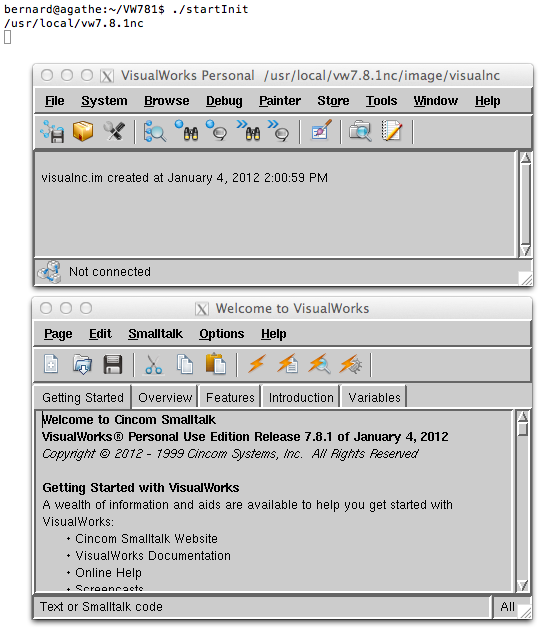
\includegraphics[width=8cm]{startInit-initialEnv.png}
\caption{Initial environment}
\label{fig:startInit-initialEnv}
\end{center}
\end{figure}
 

\section {Creating a new project }
\subsection {New image file creation }

The process of creating a new environment is reproduced for each new project. Once the initial 
environment is up, we save it to the new project name.

The trick is simply to save the image at the current location, or to a newly created directory,
thus creating a new image file. Figure 
\ref{fig:startInit-newEnv} shows an image creation Dialog opened from {\sl $File>save$ $as$} menu.
Notice the following points:
\begin{itemize}
\item Access to the current directory by the right button on the first line of Dialog.
The default location shown on the button is the VISUALWORKS home which is not suitable as a working location.

\item the image file name is changed to {\tt project1.im} to reflect the name of a new project.
\end{itemize}
After this, do a {\sl Save}, then using {\sl $File>Exit$}, quit the initial image without saving.
 
\begin{figure}[hbtp]
\begin{center} 
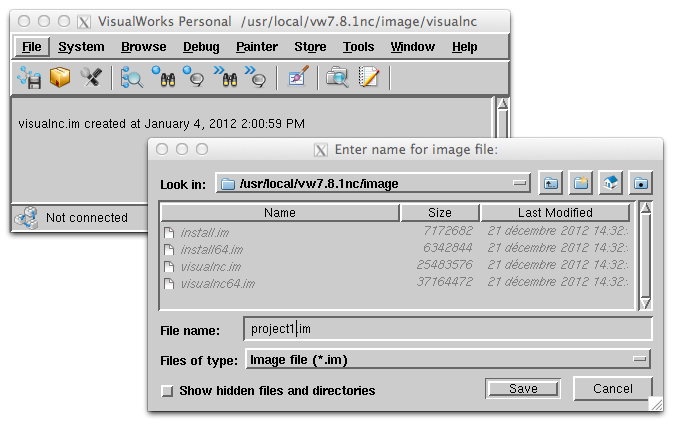
\includegraphics[width=10cm]{startInit-newEnv.png}
\caption{Creating a new image file {\sl project1.im} }
\label{fig:startInit-newEnv}
\end{center}
\end{figure}




\subsection {New script creation }

Now, we have a new file called {\sl project1.im} that we ca use to host developments.
Check its presence by listing the directory {\tt ls project1.*}. 

It is more easy and secure to setup a new script file to launch our project. So, we copy startInit to startProject1,
({\tt cp startInit startProject1}), and we modify startProject1 as follows:

\begin{lstlisting}  [language=bash,caption={bash version}]
#!/bin/bash
export VISUALWORKS=/usr/local/vw7.8.1nc
echo $VISUALWORKS
${VISUALWORKS}/bin/linux86/visual ./project1.im
\end{lstlisting}

Then, as in section \ref{sec:initialEnv}, {\tt chmod +x startProject1 ; ./startProject1}, that launch 
the new project safely.


\subsection{Summary}

\begin{itemize}
\item Creation of a directory to host developments
\item Two scripts to launch the initial environment, and to launch a new project environment
\end{itemize}

We just need to recall the files location, we can launch and quit the project, making the choice of
saving modifications to a file or not.
\section { Connecting to Store}


Once the {\sl project1} environment is launched, it becomes possible to connect to software repository.
This is done by the Store facilities in the main window. Observe the $Store$ menu.

\subsection {Accessing a repository }

Figure  \ref{fig:store-access} shows the Dialog allowing to connect to a package repository.
The menu $Store>Connect$ $Repository$ will open it. The fields are filled with location and permissions to
access the server at UBO. It is safe to save the connection to allow an easy reuse.
Connection is normally fast, and release the Store menu quickly.

\begin{figure}[hbtp]
\begin{center} 
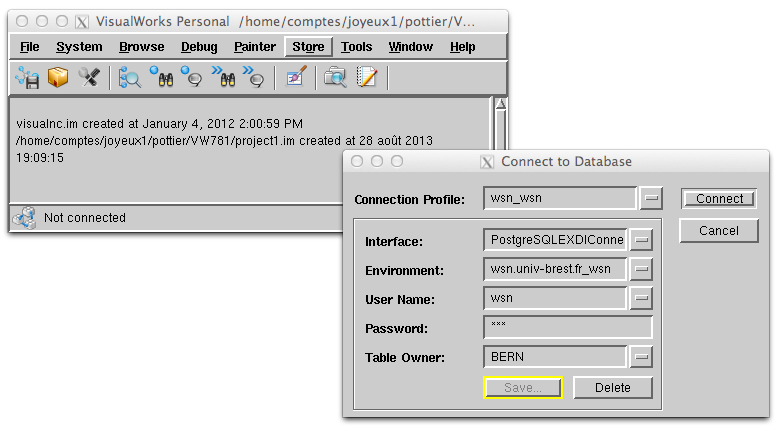
\includegraphics[width=10cm]{store-access.png}
\caption{Defining a repository access }
\label{fig:store-access}
\end{center}
\end{figure}

\subsection {Loading packages }

Once a connection is valid, by using $Store>Published$ $items$, we can observe the database contents, select
package, an load software. Figure \label{fig:store-load} shows how to proceed in the case of DistributedModeling:

\begin{enumerate}
\item select the name of a package on the left list
\item watch the different versions appearing in the right list
\item select one version
\item open the version menu and says $Load$
\end{enumerate}

\begin{figure}[hbtp]
\begin{center} 
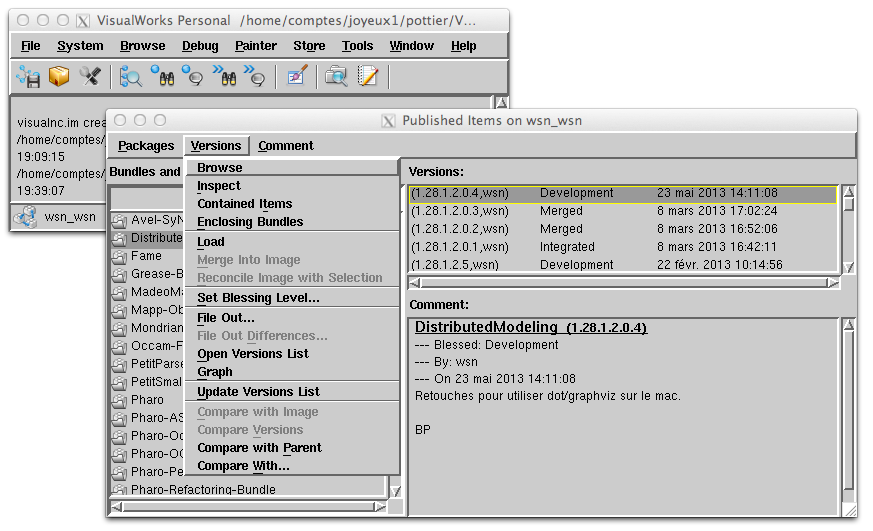
\includegraphics[width=10cm]{store-load.png}
\caption{Choosing and loading packages}
\label{fig:store-load}
\end{center}
\end{figure}

The Store tool will retrieve packages and needed dependencies from the server (if these dependencies
are correctly defined). This take time. At the end of the process, the NetGen window appears (figure  \ref{fig:netgen-initial}).
Th Hotdraw window can be closed safely, this package is of marginal interest in the project.


\subsection {Checking NetGen }
\begin{figure}[hbtp]
\begin{center} 
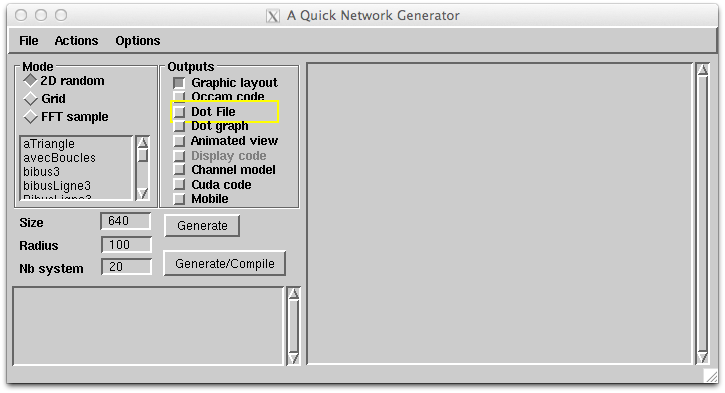
\includegraphics[width=10cm]{netgen-initial.png}
\caption{NetGen initial window }
\label{fig:netgen-initial}
\end{center}
\end{figure}

By selecting 2D Random, and Graphic layout, then by pushing the Generate button,  a random layout
of 20 systems is produced, and connections are computed based on a minimum distance of 100 points.
Figure \ref{fig:netgen-commented} shows a different case, where the number of systems has been
increased to 40. The graphic window displays the resulting layout, with 5 networks and 3 isolated nodes:
the bottom left view inside the control window states that 37 nodes are connected. 

The edges in the graph represents possible connections between nodes, given a range of 100. Grey zone figures
uncovered points, while white zones are always under control of a node.

\begin{figure}[hbtp]
\begin{center} 
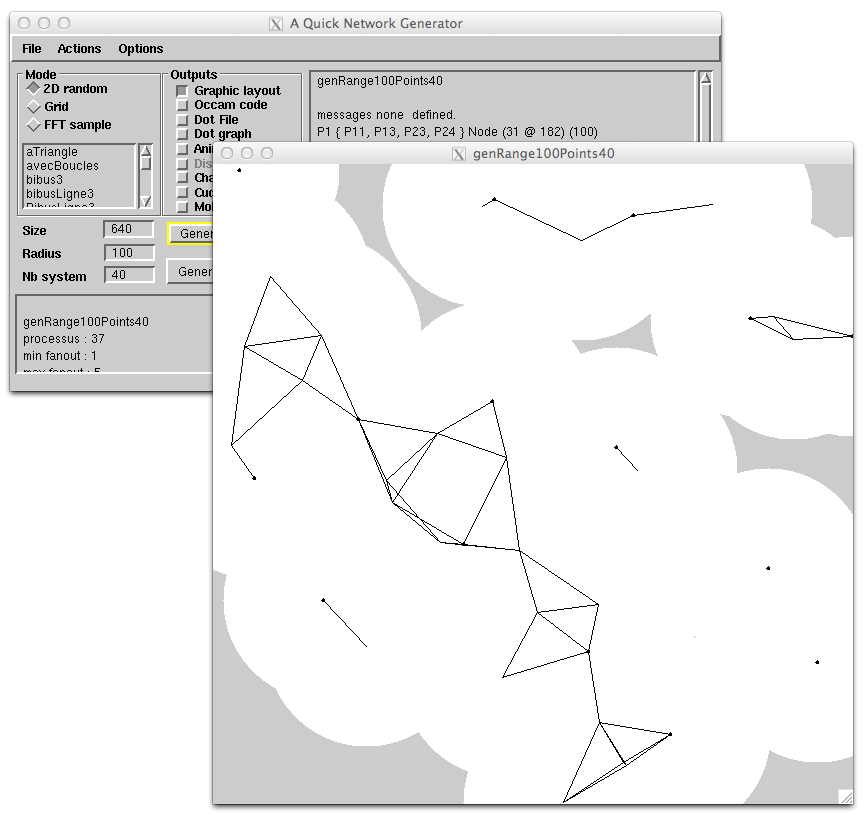
\includegraphics[width=10cm]{netgen-commented.png}
\caption{NetGen : random network generation with 40 nodes}
\label{fig:netgen-commented}
\end{center}
\end{figure}

The full statistic for this sample quantifies the graph structure in relation with a surface
where the network is produced.

\begin{lstlisting}  
genRange100Points40
processus : 37
min fanout : 1
max fanout : 5
channels   : 114
coverageArea   : 368718
percentArea   : 90
\end{lstlisting}
\section {Summary }

\subsection{Knowledge status}
At this point, it is  probably useful to save an image from the VisualWorks launcher window : $File>Save$.
Knowledge  status is :
\begin{enumerate}
\item Development tools installation for VisualWorks,
\item Connection to a package repository data base
\item Loading NetGen development tools
\item Checking NetGen functionality
\end{enumerate}

\subsection{More background, some useful tricks about Smalltalk}

\begin{itemize}
\item 
The selection of  $Tools>Workspace$ inside the main window launcher, launches an additional
window similar to a terminal. Inside this window, users can type and execute Smalltalk statements.

Execution is obtained by selecting a piece of code, calling a pop-up menu (right click), selecting 
$do it$, or $ print it$ (or $inspect$) inside this menu. Pay attention to the fact that the menu must be observed
carefully to do a selection. By releasing the $print it$ option, the code is compiled, evaluated, and 
the resulting value in variable $x$ is displayed in the Workspace.


\begin{figure}[hbtp]
\begin{center} 
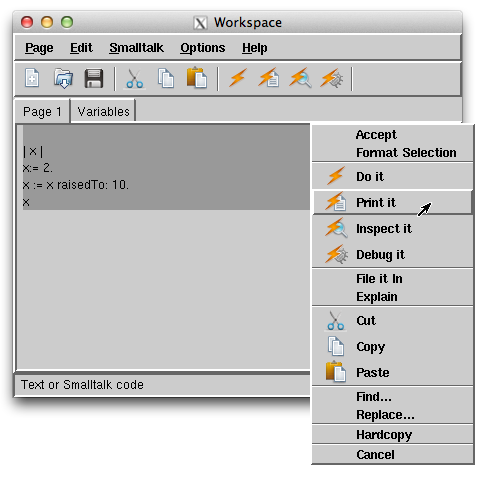
\includegraphics[width=10cm]{printIt.png}
\caption{Programming in work-spaces}
\label{fig:printIt}
\end{center}
\end{figure}
 
\item 
In a similar way, application windows can be opened, or data set can be prepared
interactively. To launch a window similar to figure \ref{fig:netgen-commented}  , type {\tt UINetworkGeometry open}
in a Workspace,
and call $do it$ from the pop-up menu.

\item 
More about Smalltalk programming : the System Workspace window (figure \ref{fig:startInit-newEnv}) gives access to lot of contributions about the
language and the system. The Smalltalk syntax is very simple, thus easy to learn: {\sl get started}\ldots 


\end{itemize}

\chapter{Building abstract networks}
\label{sec:chapter2}

Our networks are abstractions appearing basically as graphs, grouping {\sl nodes} representing  actual systems, {\sl edges} representing communication links.
Abstraction allows to cover lot of situations, from the nano scale to the universe, and lot of domains, such as distributed sensing, 
distributed computing, communication systems, environment modeling, bio systems.

Here, the focus is on wireless sensor networks design and validation in regards of practical situations in the environment.
NetGen software {\sl upper services} have the following objectives:

\begin{enumerate}
\item Practical system description based on geometry.

As example, from a map, one can decide sensor locations taking into account physical considerations, decide
on a wireless technology, and infer workable communication links.

{\sl Description can be achieved based on maps, or pictures. Alternatively, generators allow to produce 
random distributions of different characteristics. A Text input format allows to exchange network topologies with external tools. }.

\item Behaviour description.

As example, nodes will execute programs, (1) to control and sense  locally  physical phenomena, (2) 
to  contribute to the distributed system activities, such as collecting, transforming  data, sending alerts.


{\sl Behaviour description follows currently the synchronous model that use discrete time boundaries 
to make system evolutions. This technique is relevant for most of the sensor network technologies, 
as example 802.15.4, or commercial Digimesh. This is because sensor systems need to go to sleep
and wake up periodically.}.


\item Validating a system behaviour.

As example, the communication load implied by a particular topology, the latency and cost for producing
diagnostics, energy cost of a particular algorithm, risks of failures, redundancy management.

 
\item Code generation.

Systems can be huge, and the order of several thousand of nodes is reached by practical applications.
They are dynamic: critical systems are exposed to failures and mobility can be central in an application.
{\sl Simulation } is a key point in validation to measure latency delays, risks, or power consumption.
Code generation integrate local behaviours inside a network topology,   run the resulting simulation code, 
and provide diagnostics.

This is a compute intensive task where a number of steps must be executed by a number of nodes.

{\sl 
Further chapters will explain how to produce simulators for Graphic Accelerators, and for multi-threaded
execution on multi-core processors, respectively from CUDA framework (x1000 processors), and
Occam process oriented programs (x10 processors).}

\item Preparing deployment.

Once a system is validated, it is necessary to prepare an  equivalent behavior for the sensors. This is also
code generation, and can be achieved in a similar way as for simulators.
\end{enumerate}

The following sections will describe existing functionality, and known challenges.


\section{Network description}

Network is described as a graph grouping nodes and communication links. In terms of data structures,
a convenient  representation is:

\begin{itemize}
\item a global Dictionary holding nodes,
\item for each link, an input node, and an output node.
\item for each node, a name, an array of input links, and an array of output links.
\end{itemize}

This representation allows to retrieve quickly the available nodes, or a particular node,
and from that node, direct neighbors, by traversing each link.

\subsection{Textual description}

The textual representation is a reflect of this organization. It appears in the right editor of NetGen window:


\begin{itemize}
\item  a title for the network, 
\item a list of messages carried by the links, 
\item  one line for each node.

These lines are a sequence grouping
\begin{itemize}
\item  the process name,
\item the neighborhood accessible by the output links, specified between braces, and separated by commas,
\item the name of the program, or procedure executed by the node,
\item node attributes
\end{itemize}

\end{itemize}

As an illustration, the network presented  figure \ref{fig:netgen-commented}  has the following specification:
  
\begin{lstlisting}
genRange100Points40

messages none  defined. 
P1 { P11, P13, P23, P24 } Node (31 @ 182) (100)
P2 { P30 } Node (499 @ 40) (100)
P3 { P4, P6, P7, P33, P37 } Node (179 @ 338) (100)
P4 { P3, P7, P8, P31, P37 } Node (224 @ 269) (100)
P5 { P20 } Node (424 @ 306) (100)
P6 { P3, P7, P22, P33 } Node (227 @ 378) (100)
P7 { P3, P4, P6, P37 } Node (173 @ 316) (100)
P8 { P4, P22, P31, P33 } Node (293 @ 293) (100)
P9 { P10, P15, P21, P39 } Node (413 @ 601) (100)
P10 { P9, P15, P21, P39 } Node (410 @ 598) (100)
P11 { P1, P23 } Node (57 @ 112) (100)
P12 { P16, P22, P28 } Node (385 @ 440) (100)
P13 { P1, P23, P24, P37 } Node (89 @ 216) (100)
P14 { P32 } Node (269 @ 42) (100)
P15 { P9, P10, P21 } Node (350 @ 638) (100)
P16 { P12, P19, P22, P28 } Node (324 @ 448) (100)
P17 { P30, P32 } Node (368 @ 76) (100)
P18 { P38 } Node (153 @ 482) (100)
P19 { P16, P28 } Node (289 @ 513) (100)
P20 { P5 } Node (403 @ 283) (100)
P21 { P9, P10, P15, P28, P39 } Node (386 @ 558) (100)
P22 { P6, P8, P12, P16, P33 } Node (306 @ 386) (100)
P23 { P1, P11, P13, P37 } Node (108 @ 171) (100)
P24 { P1, P13, P35 } Node (18 @ 281) (100)
P25 { P29, P34, P36 } Node (580 @ 175) (100)
P28 { P12, P16, P19, P21 } Node (375 @ 487) (100)
P29 { P25, P34, P36 } Node (560 @ 152) (100)
P30 { P2, P17 } Node (420 @ 51) (100)
P31 { P4, P8 } Node (279 @ 237) (100)
P32 { P14, P17 } Node (281 @ 35) (100)
P33 { P3, P6, P8, P22 } Node (250 @ 380) (100)
P34 { P25, P29 } Node (537 @ 154) (100)
P35 { P24 } Node (41 @ 314) (100)
P36 { P25, P29 } Node (639 @ 172) (100)
P37 { P3, P4, P7, P13, P23 } Node (145 @ 255) (100)
P38 { P18 } Node (110 @ 436) (100)
P39 { P9, P10, P21 } Node (457 @ 570) (100)
\end{lstlisting}



\subsection{Logic description}
\label{sec:logicdes}
For small size networks, a logic organization can be processed by an external program called
Graphviz. On Linux system, packages are available, thus on an Ubuntu system, it should be
sufficient to load it ({\tt apt-get install graphviz}). The input of this program is expressed 
in the {\sl dot} syntax.

To produce dot files, select {\sl Dot File} option which will produce a .dot file in the directory {\sl Generated/}.
When {\sl Dot Graph} is selected, and where graphviz is available, the file is processed to produce
a postscript representation that lot of viewers can read (see Figure \label{fig:genRange100Points40-rogne}).
 

\begin{figure}[hbtp]
\begin{center} 
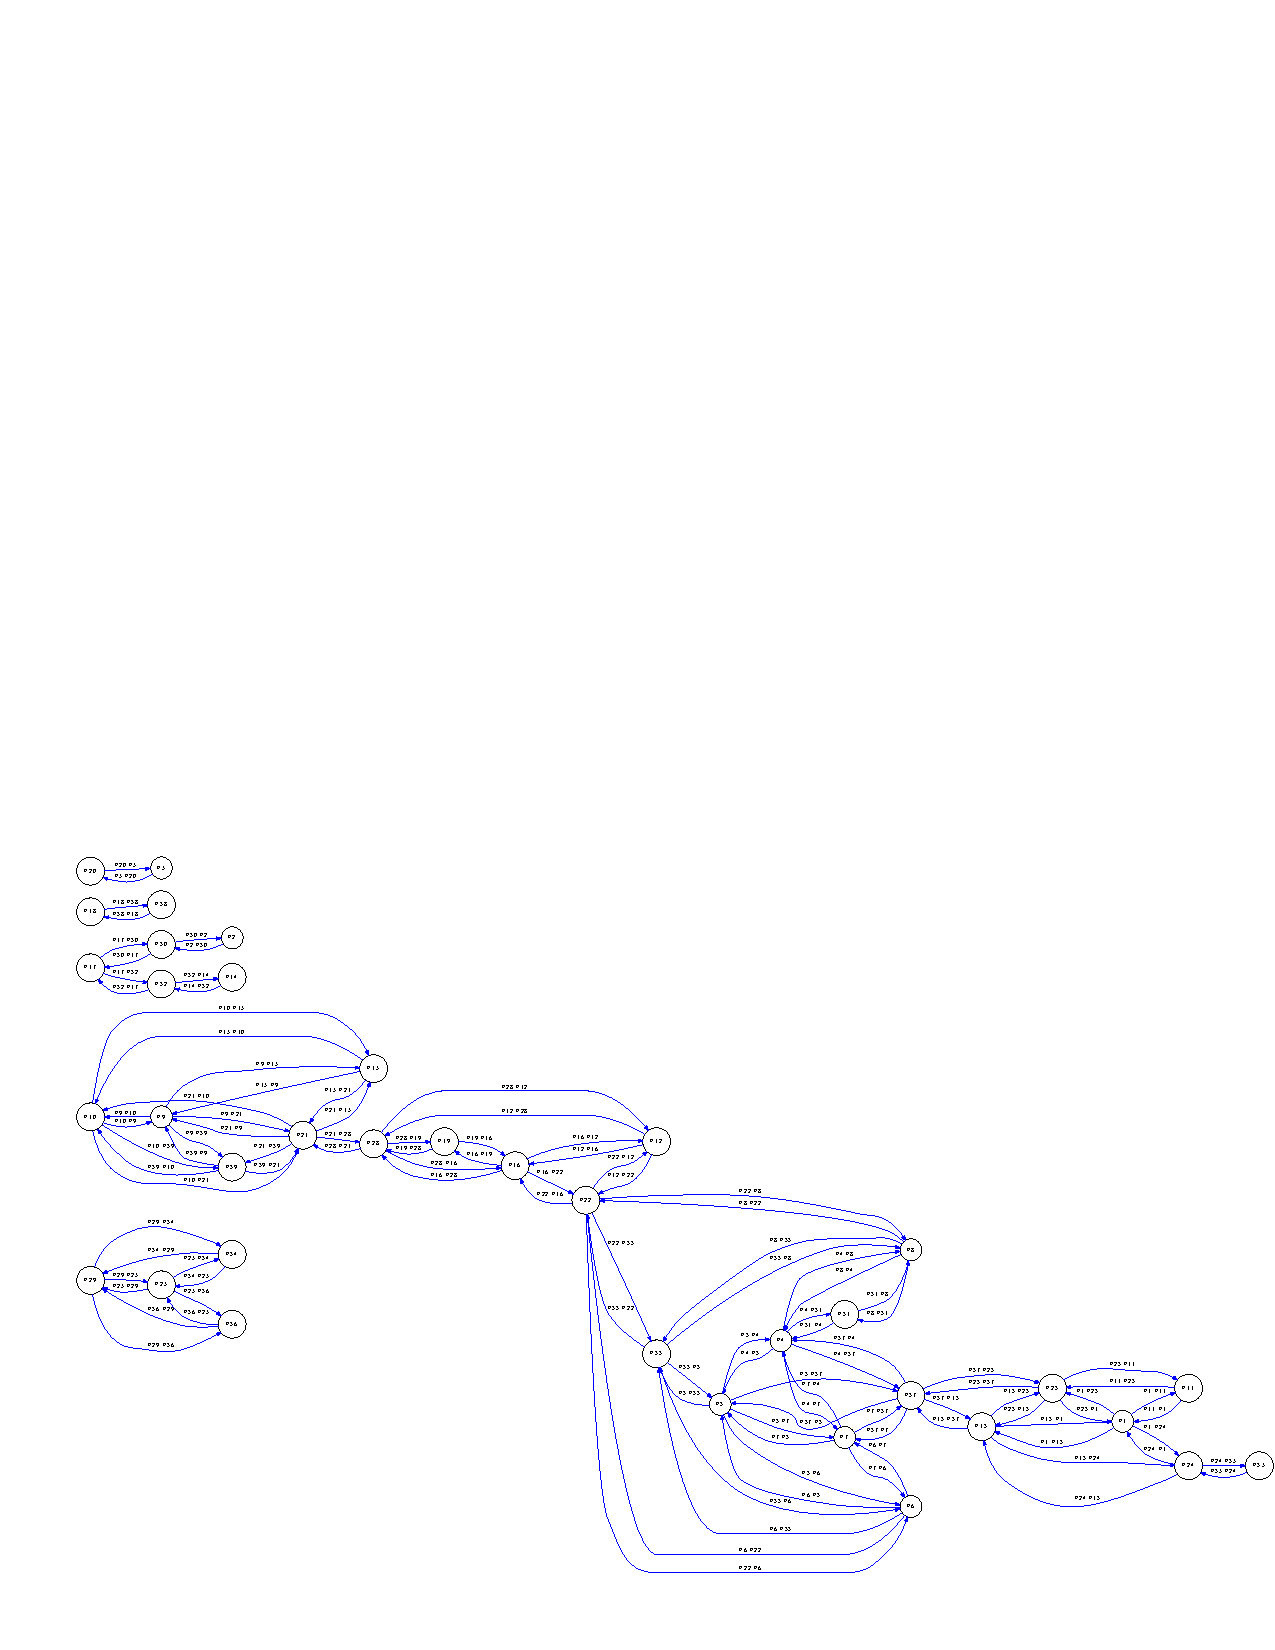
\includegraphics[width=12cm]{genRange100Points40-rogne.pdf}
\caption{Logic organization as seen in {\sl graphviz}}
\label{fig:genRange100Points40-rogne}
\end{center}
\end{figure}
 

\subsection{Programming networks, and processing}
\label{sec:ring5Def}
The control window allows to save descriptions as .net text files, and to reload saved files.
Processing these files can be done at any time by calling {\sl accept} function in 
the editing facility. This will produce Dot files, Occam programs, CUDA programs
when necessary.

The .net files can also be produced externally, specified within the editor, or the network structure
can be produced by programs. 

As a sample experiment  a directional ring with 5 Nodes is specified as follows:

\begin{lstlisting} 
ring5

messages none  defined. 
Head { P1  } Node 
P1 { P2 } Node  
P2 { P3 } Node  
P3 { P4 } Node  
P4 { Head } Node 
\end{lstlisting}

\begin{figure}[hbtp]
\begin{center} 
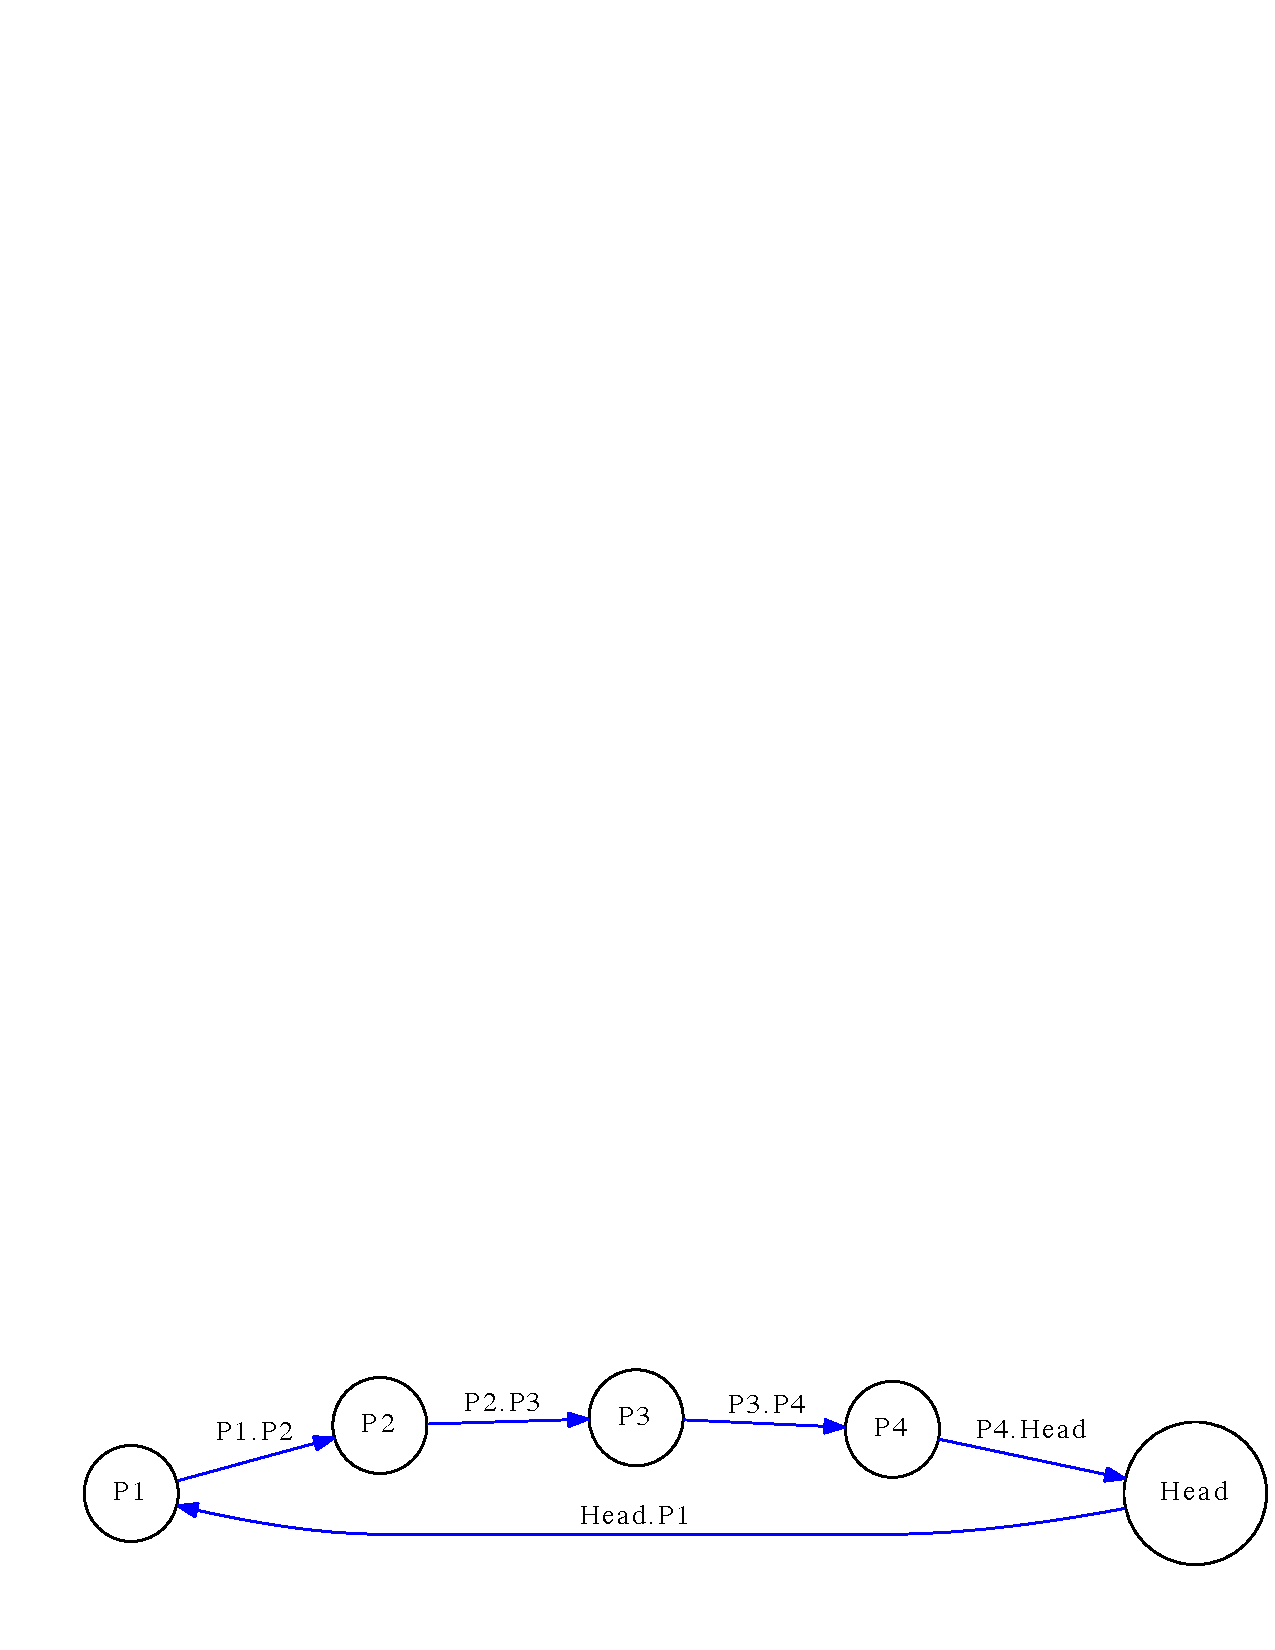
\includegraphics[width=8cm]{ring5-rogne.pdf}
\caption{Ring5}
\label{fig:ring5}
\end{center}
\end{figure}

\subsection{Building networks by program}

{\sl To be completed later.}

The section can be skipped in a first stage. it implies some Smalltalk programming: one to two pages
with pieces of listings.

\section {Regular networks}

{\sl To be completed later.}

 This function is called by selecting Grid rather than 2D Random, filling the range (200) and
number of systems (40). The connectivity is computed on this basis..


\begin{figure}[hbtp]
\begin{center} 
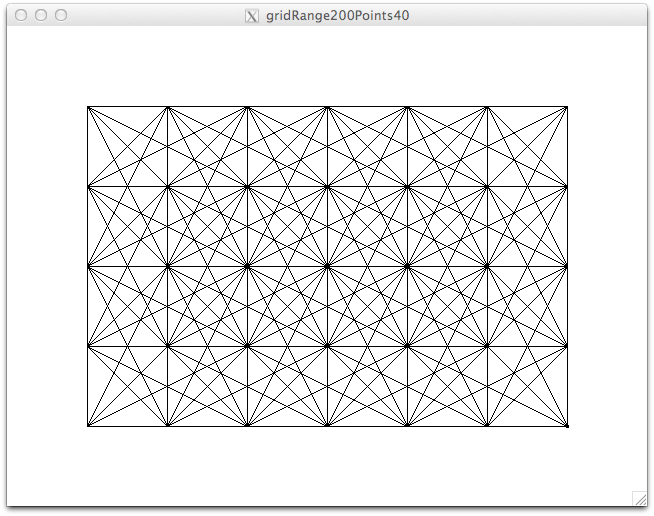
\includegraphics[width=8cm]{GridRange200Points40.png}
\caption{Layout on a rectangular surface with 200pts range and 40 nodes (at most).}
\label{fig:GridRange200Points40}
\end{center}
\end{figure}


\section{Selecting a sensor layout from a map}

Whereas the sensor network will be deployed, it is necessary to define sensing points,
and expected connectivity between these points. Ranges produced by wireless technologies
can be very different, very small for {\sl body area networks} to very large, country size applications.
Most of the solutions use dedicated network architectures that compute and route information, 
or standard solutions that support routing and sequencing of communications.
In any case, the network topology is critical for two opposite reasons:

\begin{itemize}
\item reducing the number of communications is necessary to save energy and time,

\item having enough redundancy in the routing capability is a solution in the case
of failures (nodes or communications).
\end{itemize}

The frequency, volume and data rate of communications are also   points of interest, with
critical effects for  
some applications requiring high peek bandwidth. In other cases, frequency
can be very low  
with the critical problems being  energy and costs.


We will use a medium size geographic map example to illustrate network design, 
but anything else could apply (body description, nano fabric, etc\ldots).
Figure \ref{fig:mekong} is a PNG satellite view coming from the Internet, that also displays
at the bottom left. An assumption is that a practical sensing application needs to deploy
wireless equipment to measure some environmental characteristic. We also suppose that
this equipment has been selected to work on distances suitable to implement a network.
As example, some 802,15,4 devices offer ranges from 20 to 40 km on the 900Mhz band.


\begin{figure}[hbtp]
\begin{center} 
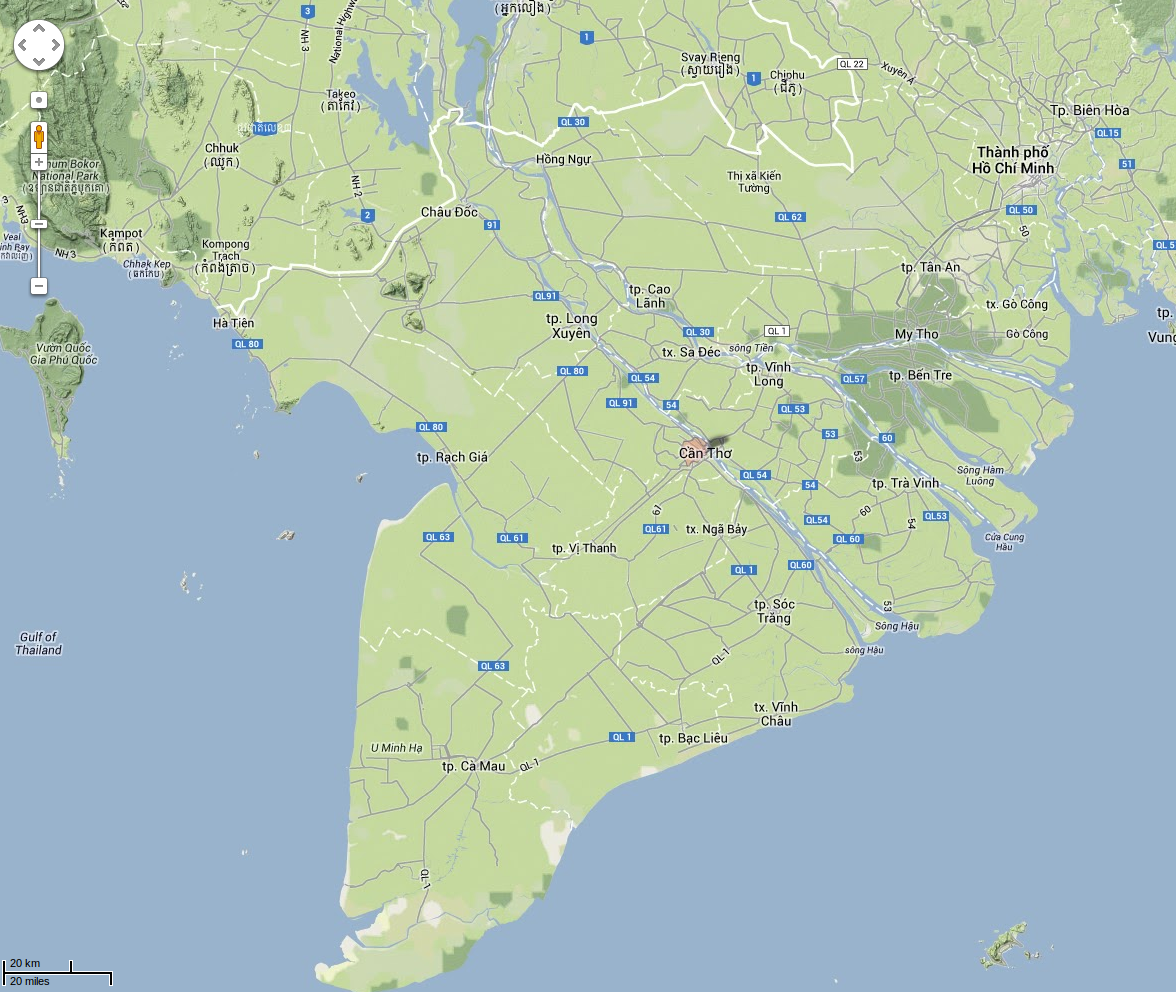
\includegraphics[width=8cm]{mekong.png}
\caption{Sample image supposed to be stored as a PNG file in the working directory.
The map has a scale useful to  tune a  range for wireless sensors.}
\label{fig:mekong}
\end{center}
\end{figure}


\subsection{Selecting sensor positions}

In NetGen control window, use the $Options>Pick$ $points$ entry to  
open a new {\sl Pick Points} window (figure \ref{fig:PickPoint1}). Then in this window, do a $File>Load$ $image$,
to load the sample image. The mouse cursor change to a cross, and each 
button pressed event will draw a circle around the selected position.




\begin{figure}[hbtp]
\begin{center} 
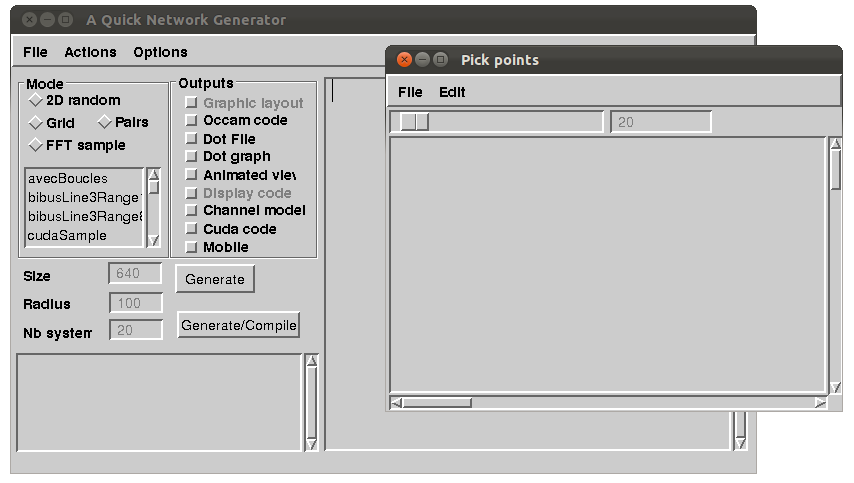
\includegraphics[width=8cm]{PickPoints1.png}
\caption{Pick point view}
\label{fig:PickPoint1}
\end{center}
\end{figure}

The slider on the top of the window, or the numeric field allow to change the range
with the effect that circles around sensors increase, or decrease. when circles
are large enough, sensors are supposed to establish radio contact ($distance(s1,s2) > range$).

A problem is to adapt the expected wireless range to the image, and a  trick
to do it is to install  fake sensor points on the scale rule (shown at the bottom of figure \ref{fig:mekong}), then to tune the slider
to obtain a communication.


\begin{figure}[hbtp]
\begin{center} 
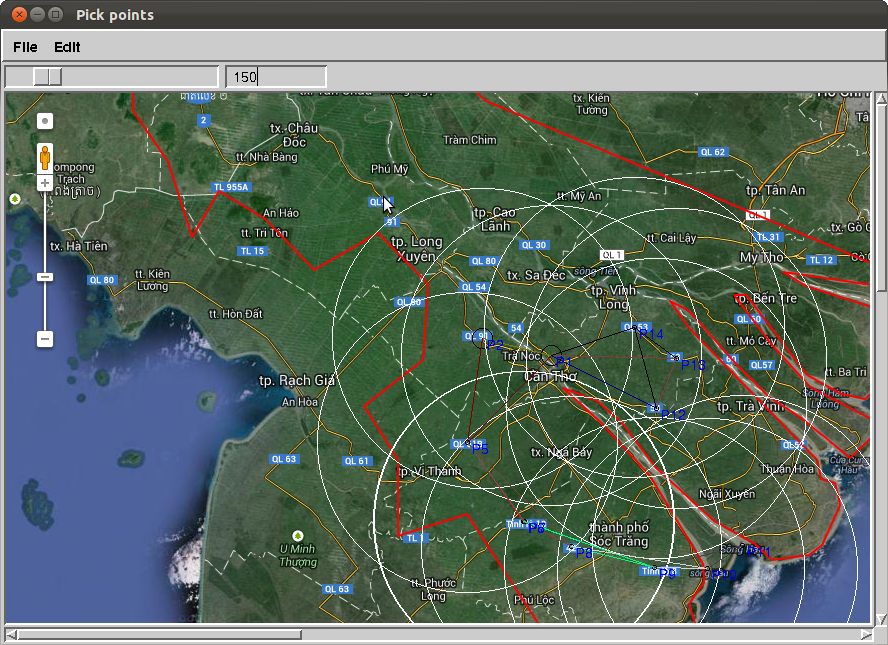
\includegraphics[width=12cm]{PickPoints3.png}
\caption{View showing sensor positions $P_i$), and connectivity.
The scale has been adapted to 150 points for a distance of 20 km.
}
\label{fig:PickPoints3}
\end{center}
\end{figure}

The $File$ menu has options   to save and reload  points position into external text files.

\subsection{Building a net}

Still in the $File$ menu, there is also a $Build net$ entry, that presents the network specification 
inside the NetGen control window (see figure 
\ref{fig:BuildNet1}).


\begin{figure}[hbtp]
\begin{center} 
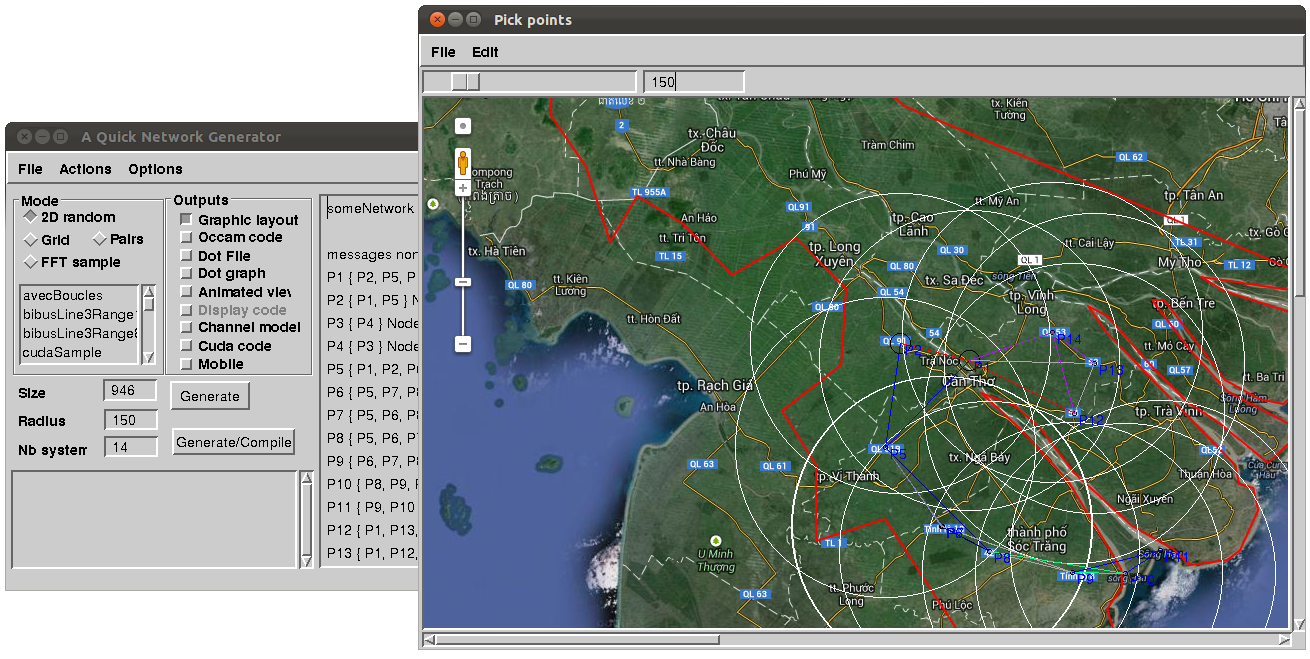
\includegraphics[width=12cm]{BuildNet1.png}
\caption{Transfer of the network to NetGen window.
}
\label{fig:BuildNet1}
\end{center}
\end{figure}

After transferring the specification, it is possible to edit it.
As example it is a good idea to change its default name.
It becomes also possible to use the code generation functions.
Figure 
\ref{fig:BuildNet2} presents a set of choice suitable for graphviz 
and Occam generation.

Notice that the call to these functions is done by the $accept$ entry
of a pop-up menu, {\sl and not the Generate button} that will destroy
the textual specification.
\begin{figure}[hbtp]
\begin{center} 
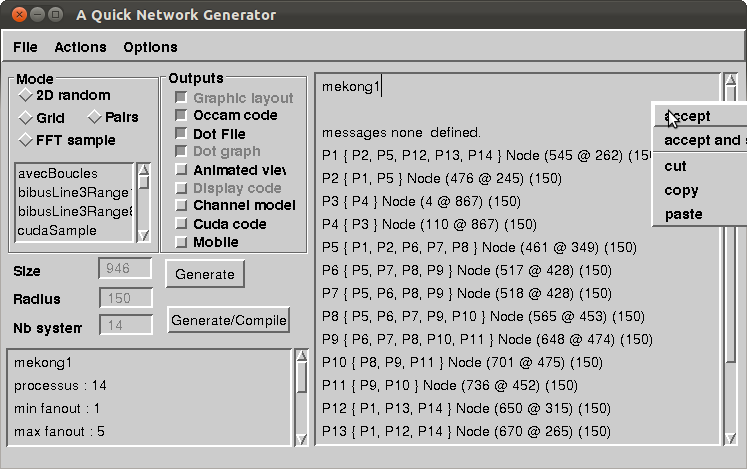
\includegraphics[width=12cm]{BuildNet2.png}
\caption{Generation of a logical network
}
\label{fig:BuildNet2}
\end{center}
\end{figure}


\subsection{Logic presentation}

The file has been dropped inside the Generated directory (section \ref{sec:logicdes})
as a Postscript file (figure \ref{fig:mekong1Logic}).
The {\sl rule fake network} appears as a parasite on the left
of the application network.

The logic file uses the same names as the $Pick Points$ view, and the textual presentation.

\begin{figure}[hbtp]
\begin{center} 
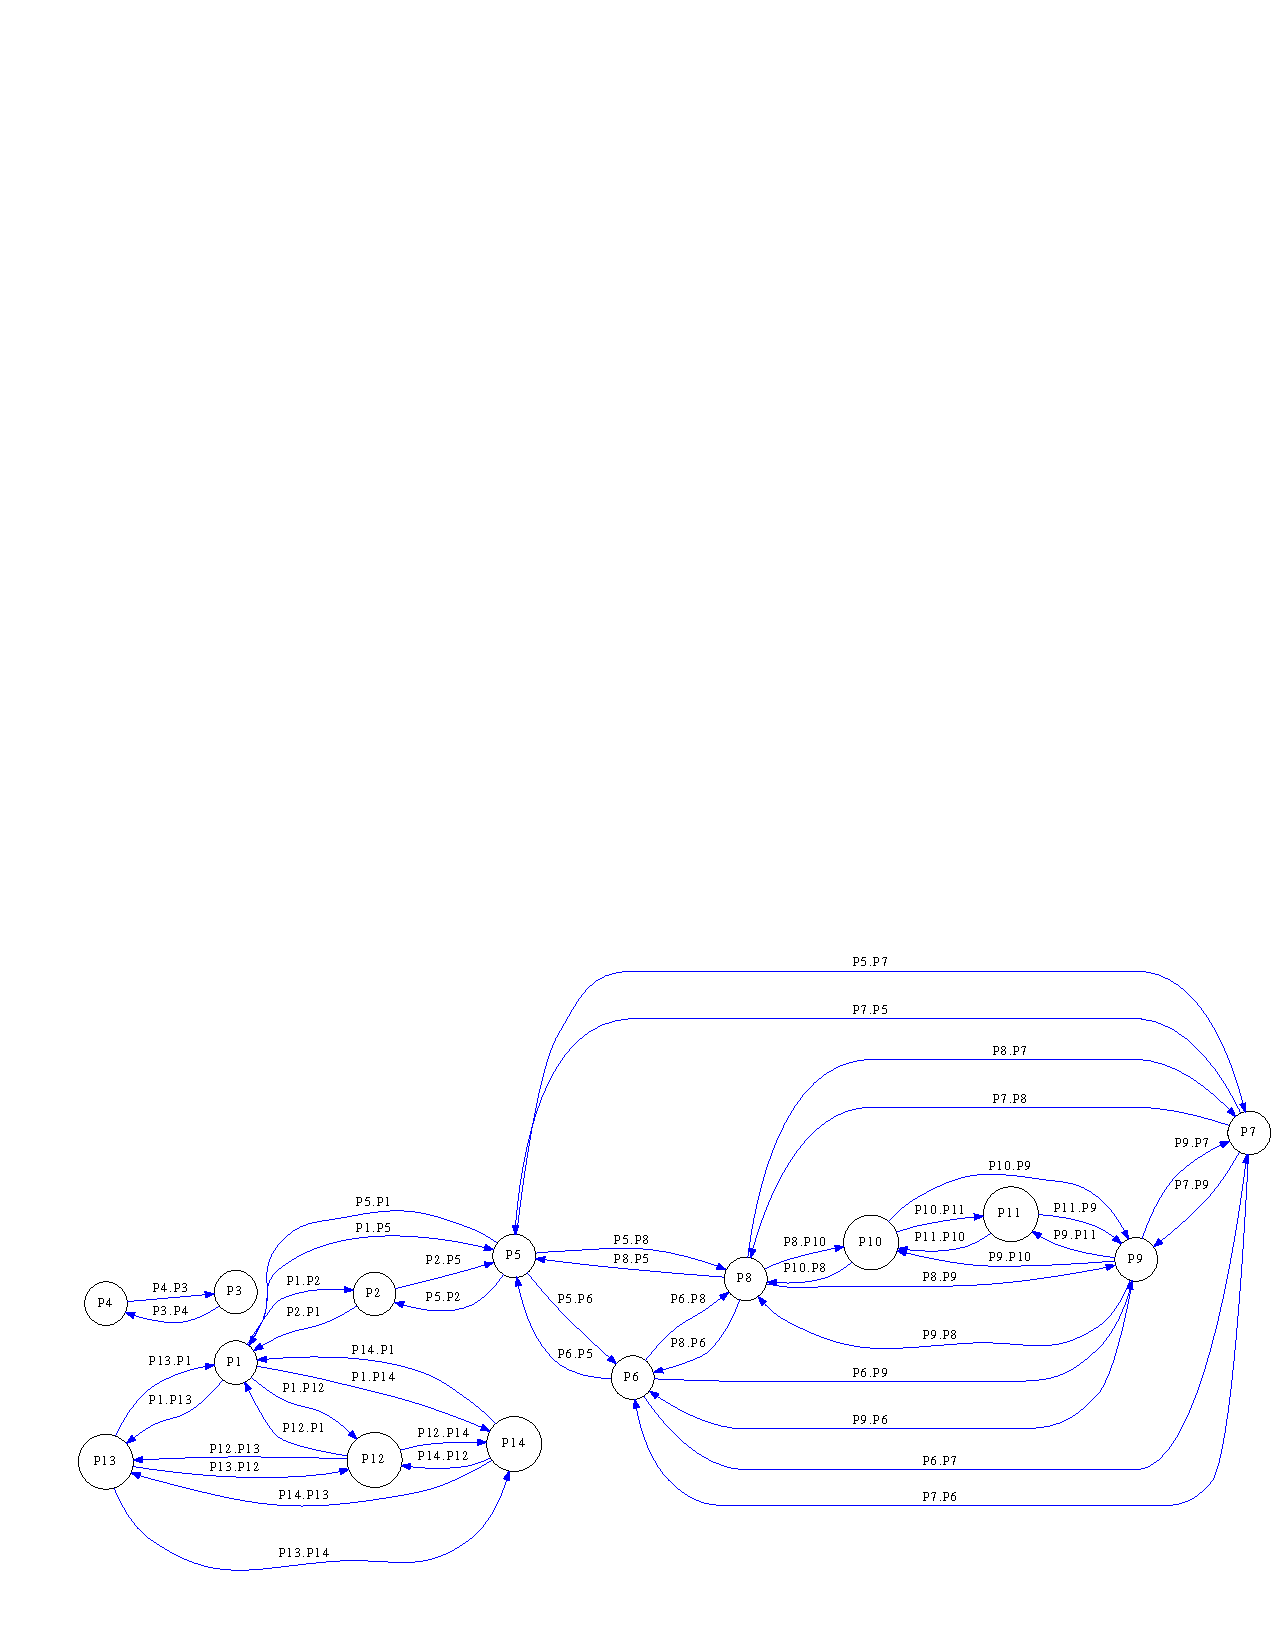
\includegraphics[width=12cm]{mekong1Logic.pdf}
\caption{Equivalent  logical network given a wireless range of 20 km
}
\label{fig:mekong1Logic}
\end{center}
\end{figure}



\section{Summary}

This chapter explains how to use maps or other images for planing sensors
positions, and how to check the topology by generating a graph view.
The Generated directory also has an architecture description file 
expressed in the Occam Syntax.



\chapter {Synchronous distributed  behaviours using Occam}

At this point, the installation of kroc, the {\sl Kent Research Occam Compiler}
should be considered. The first section will detail how to proceed on a Linux
installation.

\section{Installing kroc}

The Occam compiler is developed at University of Kent, with its home page at
{\tt http://projects.cs.kent.ac.uk/projects/kroc/trac/}.. Two branches are proposed:
out of the same compiler frontend:
\begin{itemize}
\item kroc i386 compiler which makes use of a code generator for x86, thus enabling execution
of programs on current multi-cores,
\item Transterpreter Virtual Machine (TVM), which enables execution on micro-controllers.
\end{itemize}

The two branches are good targets for wireless sensor designs. The first is used
to support concurrent simulation of networks, the second will support execution 
at sensor level in a portable way.

In this chapter, the i386 execution of simulations is the main concern, and our guide 
is the web page provided by Kent (it would be sufficient to follow these steps).
This section is just a check out of instructions provided at this location.

\begin{enumerate}
\item access installation page from {/sl Information for users}
\item check your system\\
\begin{lstlisting}
uname -a
Linux MyLinuxBox 3.2.0-51-generic #77-Ubuntu SMP Wed Jul 24 20:18:19 UTC 2013 x86_64 x86_64 x86_64 GNU/Linux
\end{lstlisting}

I have a 64bits installation supporting concurrent execution.
\begin{lstlisting} 
lsb_release -a
LSB Version:    core-2.0-amd64:core-2.0-noarch:core-3.0-amd64:core-3.0-noarch:core-3.1-amd64:core-3.1-noarch:core-3.2-amd64:core-3.2-noarch:core-4.0-amd64:core-4.0-noarch
Distributor ID: Ubuntu
Description:    Ubuntu 12.04.2 LTS
Release:        12.04
Codename:       precise
\end{lstlisting}

This is Precise 12.04 LTS distribution of Ubuntu.
\item Fetch packages dependencies useful for kroc installation on Ubuntu as explained in Debian/Ubuntu
({\sl Linux:   If you're using Debian or Ubuntu, see DebianInstallation. }). For 32bits and 64bits installation, it is:
\begin{lstlisting} 
sudo apt-get install aptitude  bash gcc binutils gawk make automake autoconf pkg-config\
libc6-dev libsdl1.2-dev libsdl-sound1.2-dev libgl1-mesa-dev   libmysqlclient15-dev libpng12-dev libxmu-dev \
libxi-dev   libplayercore2-dev libplayerc2-dev libltdl3-dev   perl python xsltproc git
\end{lstlisting} 

Additional step to support 32bits programs on 64bits systems such as MyLinuxBox:
\begin{lstlisting} 
sudo apt-get install libc6-dev-i386 lib32gcc1 gcc-multilib
\end{lstlisting} 

And we can get back to the main installation page.

\item Fetching kroc sources using git (fast):

\begin{lstlisting}  
git clone --depth 1 -b kroc-1.6 git://github.com/concurrency/kroc.git kroc-git
\end{lstlisting}  

This leaves a kroc-git additional directory with the sources. Change to this directory ({\tt cd kroc-git}).
There is a {\tt build } command to configure the compiler sources, and, as mentioned in kroc web page
one useful parameter would be to define the installation location.

\item Configuration and compilation of kroc {\sl for end users} (we are end users),  it takes time:



\begin{lstlisting}  
./build --prefix=/usr/local/kroc
\end{lstlisting}  

On MyLinuxBox, we got errors, due to wrong  installation of graphics libraries.
\begin{lstlisting} 
occbuild --in-tree /home/bernard/Documents/netgenDoc/kroc-git --toolchain=kroc --library occGL.lib --include occGL.inc  \
-lglut -lGLU -lGL  -lSM -lICE  -lX11 -lXext -lXmu -lXt -lXi    opengl_wrap.o
/usr/bin/ld: cannot find -lglut
/usr/bin/ld: cannot find -lGLU
/usr/bin/ld: cannot find -lGL
/usr/bin/ld: cannot find -lSM
/usr/bin/ld: cannot find -lICE
...
\end{lstlisting} 

A simple workaround is to start make with the ignore errors flag:
{\tt .make -i
}

And the final diagnostic was :
\begin{lstlisting} 
KRoC has now been built.

Modules enabled (33/50):
  cif convert course dblmath dynproc file fmtout forall hostio hostsp http ioconv 
maths occGL proc random raster rastergraphics rasterio rastertext selector shared_screen 
snglmath sock solib splib ss stream string time trap ttyutil useful

Modules disabled (17/50):
  button cdx cspdrv graphics3d miniraster moa netbar occSDL occSDLsound occade occplayer ocuda player pony sdlraster udc video
\end{lstlisting} 


\item Now we install the programs in /usr/local/kroc,  by typing : {\tt sudo make -i install}.

Checking the installation we see a kroc compiler, and two shell scripts to configure the environment:
\begin{lstlisting} 
 ls /usr/local/kroc/bin
ilibr kmakef kroc kroc-setup.csh kroc-setup.sh mkoccdeps occ21 occamdoc occbuild tranx86 trapns
\end{lstlisting} 

\item Obtain access to the compiler and checking access (bash version):
\begin{lstlisting} 
MyLinuxBox: $ source  /usr/local/kroc/bin/kroc-setup.sh
MyLinuxBox: $ which kroc
/usr/local/kroc/bin/kroc 
MyLinuxBox: $ echo $LD_LIBRARY_PATH
/usr/local/kroc/lib
\end{lstlisting} 

As this setup is to be done for each session, it is convenient to copy the script
inside the shell configuration file (edit {\tt ~/.bashrc}, as example).


And finally, we can launch the kroc compiler
\begin{lstlisting} 
MyLinuxBox: $  kroc
KRoC version 1.6.0 targeting x86_64-unknown-linux-gnu (driver V2.0)
Usage: kroc [options] [occam sources/pre-compiled sources]
Options:
  -b,  --brief           Give brief occ21 error messages
  -c,  --compile         Compile source to objects, do not link
  -s,  --strict          Strict checking mode
  -S,  --stoperror       Compile in STOP error mode
  -d                     Enable post-mortem debugging
  -di                    Enable insert debugging
  -e                     Enable user-defined channels
  -h,  --help            Print this message and exit
....
\end{lstlisting} 


\end{enumerate}

\section{Checking Occam compiler: Hello world! }

Samples to learn Occam programming are available under the examples directory
for each module. Basic Occam examples are accessible in ./modules/course/examples
and ./modules/course/exercises
under  the kroc-git directory.

\begin{lstlisting} 
MyLinuxBox: $ cat hello_seq_world.occ
PROC hello.world (CHAN BYTE keyboard?, screen!, error!)
  --{{{
  VAL []BYTE greeting IS "Hello World*c*n":
  SEQ i = 0 FOR SIZE greeting
    screen ! greeting[i]
  --}}}
:
\end{lstlisting} 

\begin{itemize}
\item Build your own Occam directory : {\tt mkdir ~/OccamDev }
\item Copy example files there : {\tt cp hello\_seq\_world.occ ~/OccamDev }
\item Change to this directory :  {\tt cd ~/OccamDev }
\item Compile by hand : {\tt kroc hello\_seq\_world.occ }
\item Execute : {\tt  ./hello\_seq\_world \\
Hello World
}
\end{itemize}

Below is a commented version of the program. In Occam
the program structure is defined by indentation of 2 spaces. This
is visible for the body of the procedure, starting at VAL line,
and for the loop, just below the SEQ statement.

\begin{lstlisting}  
-- start a comment
PROC hello.world (CHAN BYTE keyboard?, screen!, error!)
-- define a procedure named hello.world
-- with 3 communication links (channels carrying bytes) 
-- associated to Linux i/o standard descriptors
  --{{{
-- this was an empty comment
  VAL []BYTE greeting IS "Hello World*c*n":
-- define a constant array of bytes with a string value, including CR
  SEQ i = 0 FOR SIZE greeting
-- sequential loop starting at i=0 with length of greeting occurrences
    screen ! greeting[i]
-- output a char to the screen channel
  --}}}
:
-- end of procedure mark.
\end{lstlisting} 


\section{Parallel construct and channels in Occam}

Coming back to the topic of network simulation, this section will construct
a concurrent program suitable for the directional ring displayed figure \ref{fig:ring5}.
Each node in the ring could represent a sensor. Sensors common behaviour is to execute
an infinite loop for:
\begin{enumerate}
\item sensing, loading some status variables with values observed locally,
\item communications
\begin{enumerate}
\item sending information to direct neighbors,
\item receiving information from neighbors,
\end{enumerate}
\item sleeping for an agreed fixed period
\end{enumerate}

\subsection {Sample ring5 behaviour }

Let us start our example as a very simple program. Each sensor activity is represented
by a process, and each process executes the same program, defined as a procedure
{\tt Node.v1}. Communication links are represented by Occam channels carrying integers.
To distinguish sensor from each other, it is necessary to provide a unique identifier {\tt Identity}.

Then, as sensing is supposed to produce some result in a local variable {\tt Local.Value},
we will simply increment this variable. 

To communicate, we pass the variable to one of our next neighbor, and receive the value 
from our previous neighbor.

This {\sl behaviour} is programmed in a {\tt ring5.v1.occ} file as follows:


\begin{lstlisting}  
PROC Node.v1 (CHAN OF INT Incoming.Chan,Outgoing.Chan, VAL INT Identity)  
  INT Local.Value, Incoming.Value :
  SEQ
    Local.Value := Identity
    WHILE TRUE
      SEQ
        Local.Value := Local.Value +1 -- 1 sensing
        PAR -- 2 communication
          Outgoing.Chan ! Local.Value
          Incoming.Chan ? Incoming.Value
        SKIP -- 3 sleeping
:
\end{lstlisting} 

Notice that step 2 is programmed with a PAR construct over sending and receiving.
We don't want to define an order for activities that are concurrent. Furthermore,
programming sequential communications would lead to a dead-lock in the
simulated ring, Occam channels being blocking channels: communication is resolved
as the 2 processes reach a synchronization point.
The concurrent construct finishes with the last branch, as a {\sl barrier} condition.

To check the grammatical correctness of this program, we can add an empty 
main activity, just after the {\tt Node.v1} procedure definition:

\begin{lstlisting}  
PROC Sys(CHAN OF BYTE in,out,err)
  SEQ
    SKIP
:
\end{lstlisting}  

Then, we compile our file {\tt ring5.v1.occ}, and we execute the result:

\begin{lstlisting}  
MyLinuxBox: $ kroc ring5.v1.occ
Warning-occ21-ring5.v1.occ(17)- parameter err is not used
Warning-occ21-ring5.v1.occ(17)- parameter out is not used
Warning-occ21-ring5.v1.occ(17)- parameter in is not used 
MyLinuxBox: $  ./ring5.v1
MyLinuxBox: $ 
\end{lstlisting} 

This programs does nothing since the SKIP statement denotes an empty process.

\subsection {Sample ring5 architecture}
\label{sec:simpleRigV2}

To obtain a more convincing ring, we need to define a ring architecture having
5 nodes, and 5 communication links.
This is done by replacing the the Sys definition by a more complete one
inside a new file  {\tt ring5.v2.occ}.


\begin{lstlisting}  
PROC Sys(CHAN OF BYTE in,out,err)
  -- channels definition
  CHAN OF INT P1.P2, P2.P3, P3.P4, P4.P5, P5.P1:
  -- concurrent ring construct
  PAR
    Node.v1 (P5.P1,P1.P2,1)  -- P1
    Node.v1 (P1.P2,P2.P3,2)  -- P2
    Node.v1 (P2.P3,P3.P4,3)  -- P3
    Node.v1 (P3.P4,P4.P5,4)  -- P4
    Node.v1 (P4.P5,P5.P1,5)  -- P5
:
\end{lstlisting} 

Now we compile and execute. This will produce a program with an infinite loop
to be killed. Notice that each channel is used 2 times,  in   input and output parameter
positions. Kroc check correctness of the architecture with two user process for
reading and writing.

\begin{lstlisting}  
MyLinuxBox: $ kroc ring5.v2.occ
Warning-occ21-ring5.v2.occ(19)- parameter err is not used
Warning-occ21-ring5.v2.occ(19)- parameter out is not used
Warning-occ21-ring5.v2.occ(19)- parameter in is not used
MyLinuxBox: $ ./ring5.v2
\end{lstlisting} 

\subsection {Ring 5 has a synchronous behaviour}

Each process has its own control loop, but the PAR communication implementation
guarantees that none of them can take much progress against the neighbors. Every 
process is in the same turn as the other ones.

The simulation is executed under Occam micro-kernel controller called CCSP,
that can be multi threaded and distributed on several processor cores.
The behaviour is semantically equivalent to what happens in a wireless network
whatever is the protocol used in the MAC layer (time division TDMA, CSMA,
acknowledged or not).

This simulation also obeys to synchronous distributed algorithms methodology,
that bring lots of opportunities for defining how the sensor network will
implement services and overcome difficulties.

\section{Observing execution, simulation traces}

The program in section \ref{sec:simpleRigV2} does not produce any
usable output. To allow observation of its behaviour, we need 
some external print out on what is happening.

Unfortunately, printing in text on a terminal requires sharing the terminal,
thus synchronization of processes willing to print. This can be overcome 
with graphics presentation, but let us see what we can do about sharing i/os.

We have seen section  that Occam program have channels mapped on
file descriptors. In the case of Ring5, the {\tt stdout} descriptor must be
written by our 5 processes. This is achieved by a multiplexer, and there
is the ALT construct of Occam that allows to take into account 5 channels
selecting one of them which appears to be ready.

ALT has an entry for channel to be inspected. A ready channel value
is read in a variable, an after this, an action is taken.
As an example let us send two channels {\tt c.in.1 c.in.2} into one channel
 {\tt c.out} :


\begin{lstlisting} 
CHAN OF BYTE c.in.1, c.in.2, c.out:
BYTE char:
SEQ i=0 FOR MaxTurns
  ALT
    c.in.1 ? char
      c.out! char
    c.in.2 ? char
      c.out! char
\end{lstlisting} 


\begin{figure}[hbtp]
\begin{center} 
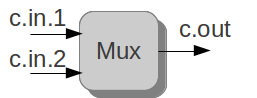
\includegraphics[width=6cm]{mux2.png}
\caption{Multiplexer on 2 channels
}
\label{fig:mux2}
\end{center}
\end{figure}

Normally, the construct is non determinist, meaning that one channel
is selected at random. Also, only one of the ready channels is taken
for each resolved ALT, and the construct block until one of its entry is ready.


\subsection {Programming a trace multiplexer }
\label{sec:ring5mux}
The procedure Mux below shows a construct for 
a fixed number of nodes (MaxNodes) looping
synchronously MaxTurns times.

\begin{lstlisting} 
#USE "course.lib"
-- enables to use formatted printing procedures, out.number(..)
VAL INT MaxNodes IS 5:
-- we have 5 nodes

VAL INT MaxTurns IS 10:
-- we will do 10 rounds

-- Mux is our observer in the system 
PROC Mux([]CHAN OF BYTE muxTab, CHAN OF BYTE out)
-- muxTab is an array of input channels
-- its size is managed by the Occam compiler
-- out is the output channel
  BYTE char:  
-- input char
  SEQ i=0 FOR  (MaxNodes * MaxTurns)
    ALT i=0 FOR SIZE muxTab
-- fetch the real size of the array
      muxTab[i] ? char
-- block until one of the input is ready
-- i is the index of the selected ready channel
        SEQ 
          out.number(i,4,out)
          -- print the index of the channel  
           out ! '*t'
          -- print a tab
         out ! char
          -- print the char
          WHILE char <> '*n'
          -- loop to the end of the line
            SEQ
              muxTab[i] ? char
              out ! char
              -- read char on the channel and print it
:
\end{lstlisting} 

This code is suitable to trace MaxNodes nodes, each of them
writing on an entry of a table, a full line closed by an end of line.
 
\subsection {Ring behavior with a  trace }
\label{sec:ring5behav}
As we want to watch what is happening in each process, we need to
add a channel to the Mux into each process, and to use this
channel inside the internal loop. As we have restricted the Mux to MaxTurns
rounds, we also need to exchange the infinite loop to 
a restricted sequence. This is the modified Node.v2 procedure:


\begin{lstlisting}  
PROC Node.v2 (CHAN OF INT Incoming.Chan,Outgoing.Chan, VAL INT Identity, CHAN OF BYTE To.Mux)  
  INT Local.Value, Incoming.Value :
  SEQ
    Local.Value := Identity
    WHILE TRUE
      SEQ
        Local.Value := Local.Value +1 -- 1 sensing
        PAR -- 2 communication
          Outgoing.Chan ! Local.Value
          Incoming.Chan ? Incoming.Value
        SKIP -- 3 sleeping
        out.number(Local.Value,0,To.Mux)
        To.Mux ! '*n'
        -- trace the value of the local variable and send CR
:
\end{lstlisting} 

\subsection {Ring architecture with trace multiplexer }
\label{sec:ringArchiv3}

Now we implement the full program with:
\begin{enumerate}
\item Mux procedure as shown section \ref{sec:ring5mux}, then
\item Node procedure from section \ref{sec:ring5behav}
\end{enumerate}

And we need to complete the process system from section \ref{sec:simpleRigV2} by declaring channels from processes to the trace collector,
and add these channels in the parallel construct branches. It is also needed to call the Mux with
its array of input channels and the system stdout access (see figure 
\ref{fig:mux3}):


\begin{lstlisting}  
PROC Sys(CHAN OF BYTE in,out,err)
  -- channels definition
  CHAN OF INT P1.P2, P2.P3, P3.P4, P4.P5, P5.P1:
  [MaxNodes] CHAN OF BYTE To.Mux.Tab:
  -- concurrent ring construct
  PAR
    Mux(To.Mux.Tab,out)
    Node.v2 (P5.P1,P1.P2,1,To.Mux.Tab[1-1])  -- P1
    Node.v2 (P1.P2,P2.P3,2,To.Mux.Tab[2-1])  -- P2
    Node.v2 (P2.P3,P3.P4,3,To.Mux.Tab[3-1])  -- P3
    Node.v2 (P3.P4,P4.P5,4,To.Mux.Tab[4-1])  -- P4
    Node.v2 (P4.P5,P5.P1,5,To.Mux.Tab[5-1])  -- P5
:
\end{lstlisting} 

The source can be compiled asking a link with the course library, 
then executed filtering the 10 first lines.
 
\begin{lstlisting} 
MyLinuxBox $ kroc -lcourse ring5.v3.occ
Warning-occ21-ring5.v3.occ(53)- parameter err is not used
Warning-occ21-ring5.v3.occ(53)- parameter in is not used
MyLinuxBox $ ./ring5.v3 | head -10
   4    6
   0    2
   1    3
   2    4
   0    3
   1    4
   3    5
   4    7
   2    5
   0    4
\end{lstlisting} 


\begin{figure}[hbtp]
\begin{center} 
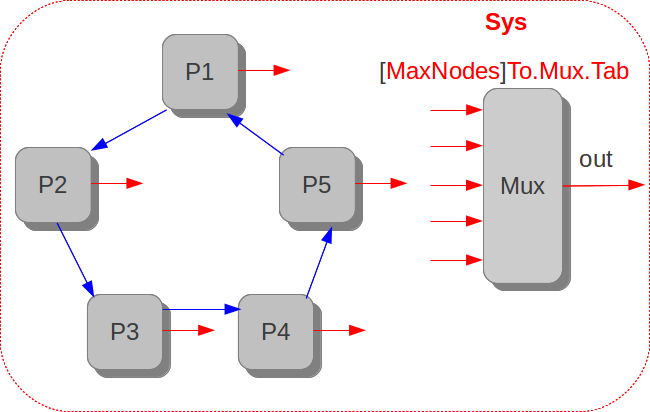
\includegraphics[width=8cm]{mux3.png}
\caption{Complete Ring5 architecture with trace multiplexer
}
\label{fig:mux3}
\end{center}
\end{figure}


If we want to see the sequence of numbers output by node 1,
we can use grep to filter this node as well:

\begin{lstlisting} 
MyLinuxBox $  ./ring5.v3 | grep '^ *1' 
   1    3
   1    4
   1    5
   1    6
   1    7
   1    8
   1    9
   1    10
   1    11
   1    12
\end{lstlisting} 

\section{Architectures and Behaviors in NetGen framework}

In section \ref{sec:ring5Def} we have shown how to produce graphs, and Occam
description too. It is time to come back to the initial ring example and to watch what 
comes out from the generator. The files produced describes architectures in a generic
way. Whatever is the network, we should be able to run our distributed behavior on it.
The {\tt Generated/} directory contains the ring architecture in the {\tt ring5.occ} file.
Let us comment its contents in a simplified way.

\subsection{Occam architecture description from NetGen}

There are 2 major differences with code detailed  in section \label{sec:ringArchiv3}:
\begin{itemize}
\item the program has been split in 2 files, one for architecture {\tt ring5.occ}, and one
for behavior  {\tt nodes-test-include.occ}. The first one (generated) includes the second one
(written by hand).
\item instead of listing all the channels in procedure parameters, we group them into
tables, and pass these tables as parameters. PROC Ring5 thus define input and output
group of channels, and pass them when starting the process:

\begin{lstlisting} 
  Head.out IS [ Head.P1 ]:
  Head.in IS [ P4.Head ]:
  -- and later
  Node(Head.in, Head.out,0, toMux [0])
\end{lstlisting} 

A big advantage in doing this is that we can have different connectivity
for different processes, and the connectivity can become very large.

This will be demonstrated later on large network examples.
\end{itemize}

\begin{lstlisting} 
#USE "course.lib"  -- support for printing
VAL INT MaxFanOut IS 1: --max number of channels per node
VAL INT MaxNodes IS 5: -- max number of nodes

#INCLUDE "nodes-test-include.occ"
-- includes the file where the behaviour is located
-- this file must contains definitions for procedures Node and Mux
-- plus the diam.proto type for communication links

PROC ring5(CHAN OF BYTE stdin, stdout, stderr)
   -- Channel declarations
  CHAN OF diam.proto Head.P1:
  CHAN OF diam.proto P1.P2:
  CHAN OF diam.proto P2.P3:
  CHAN OF diam.proto P3.P4:
  CHAN OF diam.proto P4.Head:

  -- Channel table declaration for nodes
  Head.out IS [ Head.P1 ]:
  Head.in IS [ P4.Head ]:
  P1.out IS [ P1.P2 ]:
  P1.in IS [ Head.P1 ]:
  P2.out IS [ P2.P3 ]:
  P2.in IS [ P1.P2 ]:
  P3.out IS [ P3.P4 ]:
  P3.in IS [ P2.P3 ]:
  P4.out IS [ P4.Head ]:
  P4.in IS [ P3.P4 ]:

  -- Program Body
  [MaxNodes]CHAN OF BYTE toMux:
  PAR
    Node(Head.in, Head.out,0, toMux [0])
    Node(P1.in, P1.out,1, toMux [1])
    Node(P2.in, P2.out,2, toMux [2])
    Node(P3.in, P3.out,3, toMux [3])
    Node(P4.in, P4.out,4, toMux [4])
    Mux(toMux,stdout)
     -- End of program body
:
\end{lstlisting} 
 
\subsection {Behaviour description, first approach }

We know copy our previous behavior in a  {\tt nodes-test-include.occ}, and noticing
that we receive array of channels, we modify the Node procedure, using the
first entry of these arrays.

It is also necessary to declare a  {\tt diam.proto} type as being an INT, and
to edit the Node procedure with cast and correct declaration of variables.

This is a first version of the behavior file:
\begin{lstlisting}
DATA TYPE diam.proto IS INT:
VAL INT MaxTurns IS 10:

PROC Mux([]CHAN OF BYTE muxTab, CHAN OF BYTE out)
  BYTE char:  
  SEQ i=0 FOR  (MaxNodes * MaxTurns)
    ALT i=0 FOR SIZE muxTab
      muxTab[i] ? char
        SEQ 
          out.number(i,4,out)
          out ! '*t'
          out ! char
          WHILE char <> '*n'
            SEQ
              muxTab[i] ? char
              out ! char
:

PROC Node([]CHAN OF diam.proto Incoming.Chan,Outgoing.Chan, VAL INT Identity, CHAN OF BYTE To.Mux)  
  INT Local.Value: 
  diam.proto Incoming.Value:
  SEQ
    Local.Value := Identity
    SEQ i=0 FOR MaxTurns 
      SEQ
        Local.Value := Local.Value +1 -- 1 sensing
        PAR -- 2 communication
          Outgoing.Chan[0] ! (diam.proto Local.Value)
          Incoming.Chan[0] ? Incoming.Value
        SKIP -- 3 sleeping
        out.number(Local.Value,0,To.Mux)
        To.Mux ! '*n'
        -- trace the value of the local variable
: 
\end{lstlisting} 

The file to compile is the architecture, the execution produces the same result as in section 
\ref{sec:ringArchiv3}.

\begin{lstlisting} 
MyLinuxBox $ ls
nodes-test-include.occ  ring5.occ
MyLinuxBox $ grep INC  ring5.occ
#INCLUDE "nodes-test-include.occ"
bernard@PedelBP:~/Documents/netgenDoc/Ring5$ kroc -lcourse ring5.occ
Warning-occ21-ring5.occ(34)- parameter stderr is not used
Warning-occ21-ring5.occ(34)- parameter stdin is not used
MyLinuxBox $ ./ring5 | head -8
   4    5
   0    1
   1    2
   2    3
   0    2
   1    3
   3    4
   4    6
\end{lstlisting} 

\section {Summary : flow for generated bidirectional ring }
Let us review specification and architecture code generation on the case of 
a bidirectional 4 nodes ring. We will need to modify  the behavioral part of the 
program, and will be ready for final statements on using  code generation
for any network.

\subsection {Specification and drawing }

This network will be called BiDirRing4. It is processed in the same way as section \ref{sec:ring5Def},
asking for Occam generation and graphviz generation.

\begin{lstlisting} 
BiDirRing4
messages none  defined. 
P1 { P2, P4 } Node
P2 { P3, P1 } Node 
P3 { P4, P2  } Node  
P4 { P1, P3  } Node  
\end{lstlisting} 


\begin{figure}[hbtp]
\begin{center} 
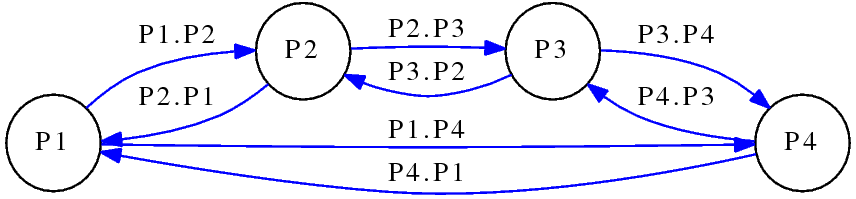
\includegraphics[width=8cm]{BiDirRing4.png}
\caption{Logic organization for 4 nodes Bi-directional ring}
\label{fig:BiDirRing4}
\end{center}
\end{figure}


\subsection {Occam resulting architecture}

The Generated directory contains the architecture description {\tt BiDirRing4.occ} from which is extracted
the code below (shortened). One can notice that channel arrays now contain 2 links rather than one
({\tt   P1.out IS [ P1.P2,P1.P4 ]:}).

\begin{lstlisting} 
-- processus : 4
-- min fanout : 2
-- max fanout : 2
-- channels   : 8
 
#USE "course.lib"


VAL INT MaxFanOut IS 2:
VAL INT MaxNodes IS 4:

#INCLUDE "nodes-test-include.occ"

PROC BiDirRing4(CHAN OF BYTE stdin, stdout, stderr)
   -- Channel declarations
  CHAN OF diam.proto P1.P2,P1.P4:
  CHAN OF diam.proto P2.P3,P2.P1:
  CHAN OF diam.proto P3.P4,P3.P2:
  CHAN OF diam.proto P4.P1,P4.P3:

  -- Channel table declaration for nodes
  P1.out IS [ P1.P2,P1.P4 ]:
  P1.in IS [ P2.P1,P4.P1 ]:
  P2.out IS [ P2.P3,P2.P1 ]:
  P2.in IS [ P1.P2,P3.P2 ]:
  P3.out IS [ P3.P4,P3.P2 ]:
  P3.in IS [ P2.P3,P4.P3 ]:
  P4.out IS [ P4.P1,P4.P3 ]:
  P4.in IS [ P1.P4,P3.P4 ]:

  -- Program Body
  [MaxNodes]CHAN OF BYTE toMux:
  PAR
    Node(P1.in, P1.out,0, toMux [0])
    Node(P2.in, P2.out,1, toMux [1])
    Node(P3.in, P3.out,2, toMux [2])
    Node(P4.in, P4.out,3, toMux [3])
    Mux(toMux,stdout)
     -- End of program body
:
\end{lstlisting} 

\subsection{General formulation for behavior}

The need is to show how to read and write several channels
rather than one. To allow this, it is needed to provide as many buffers
as there are input and output links. The maximum connectivity in
the network is known in a constant MaxFanOut. Thus, we can dimension and
control these buffers.

As we are sending from buffers, it is also necessary to copy state values,
or produce messages in the buffers, and similarly, we will need to collect
and examine incoming messages to update node status.

Data type diam.proto, and procedure Mux does not change.
An updated Node procedure appears as follows in a new version of {\tt nodes-test-include.occ}:

\begin{lstlisting} 
PROC Node([]CHAN OF diam.proto Incoming.Chan,Outgoing.Chan, VAL INT Identity, CHAN OF BYTE To.Mux)  
  [MaxFanOut] INT Local.Values:  -- buffers for outgoing messages
  [MaxFanOut] diam.proto Incoming.Value: -- buffers for incoming
  INT Local.Value:
  SEQ
    Local.Value := Identity
    SEQ i=0 FOR MaxTurns 
      SEQ
        Local.Value := Local.Value +1 -- 1 sensing
        SEQ i=0 FOR MaxFanOut -- copy our state to outgoing buffers
          Local.Values[i]:= Local.Value
        PAR -- 2 communication
          PAR index = 0 FOR MaxFanOut -- send in parallel
            Outgoing.Chan[index] ! (diam.proto Local.Values[index])
          PAR index = 0 FOR MaxFanOut -- receive in parallel
            Incoming.Chan[index] ? Incoming.Value[index]
        out.number(Local.Value,0,To.Mux) -- trace some state
        To.Mux ! '*n'
:
\end{lstlisting} 

Compile and execute in a specific directory {\tt BiDirRing4}:

\begin{lstlisting} 
MyLinuxBox $ ls
BiDirRing4  BiDirRing4.occ  nodes-test-include.occ
MyLinuxBox $ kroc -lcourse BiDirRing4.occ
Warning-occ21-BiDirRing4.occ(32)- parameter stderr is not used
Warning-occ21-BiDirRing4.occ(32)- parameter stdin is not used
MyLinuxBox $ ./BiDirRing4 | head -6
   3    4
   0    1
   1    2
   2    3
   0    2
   1    3
\end{lstlisting} 

\subsection {Exercise }

Verify that you can produce a trace for an 8 nodes bidirectional ring
for the same behaviour..


\subsection {Exercise }

BiDirRing4 is not a good demonstration of cooperation between nodes
since the program ignores values in incoming messages. A step forward
would be to compute mean of a value distributed in the neighborhood:

\begin{itemize}
\item modify BiDirRing4 to send a local value to the direct neigbors
\item receive values from the neigbors and compute the mean of these values
including the local one.
\item repeat the process for neighborhoods of 5 nodes inside the ring.
Do  a trace analysis.
\end{itemize}


\chapter{Distributed algorithms simulation}

Be fore developing actual programs for wireless sensor networks, it
is good to check if the cooperation of local programs will lead
to working and efficient results.

The distributed behaviour comes from:

\begin{itemize}
\item an architecture specification, such as {\tt mekong1.occ},
\item a behaviour executed by nodes, such as {\tt nodes-test-include.occ}.
\end{itemize}

The two descriptions are orthogonal, meaning that one can make
evolution on the architecture at fixed behaviour, or make evolutions on
the behaviour with fixed architecture. The situation is well known
in computer architecture. It is named an Y methodological approach,
and was popularized by Gajski.
The bottom branch carrying measures produced from tools (energy, 
response time, cost, etc\ldots).




\chapter{A NetGen-compatible map browser}

This chapter will present two evolutions of the initial Netgen program for 
support of precise geographic positions and map browsing, then for displaying 
buildings or obstacles representations extracted from OpenStreetMap databases. 
The present tools allow to interact with the more common public information systems 
such as Google map and OpenStreetMap. 

The map browser is a tool allowing to display various kind of maps and to represent 
locations of interest such as sensors set in the country. 
As this tool is developped on the same platform as NetGen, the procedures described 
in chapter \ref{sec:chapter1} will apply to access the software: 
\begin{itemize}
\item start a fresh image and ensure that the NetGen package is loaded with one of the last 
version (1.28.1.2.5 should work)
\item open the store dialog from VisualWorks main window
\item select GoogleMap package (we need to change this name)
\item select version 1.15.5.2 or later, and type load from the pop-up menu
\end{itemize}

The initial window displays as show figure \ref{fig:initialGmap}. 

\begin{figure}
\begin{center} 
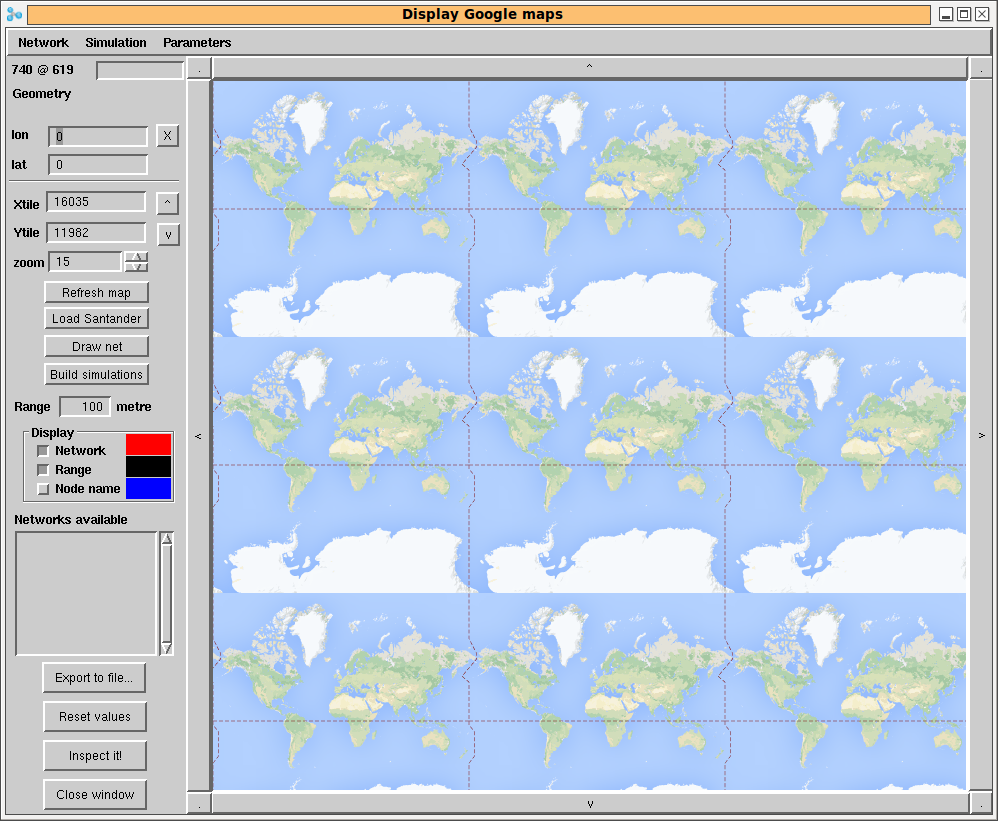
\includegraphics[width=8cm]{gmap.png}
\caption{Initial view on the map browser: the right part displays tiles from the map 
from public servers. The left column displays geographic information and allows 
to control network presentation. }
\label{fig:initialGmap}
\end{center}
\end{figure}

\section{Moving on the map}
A predefined position is visible inside the xtile and ytile fields 
in the left column of the browser. Just below, a zoom factor is also provided. 
Whatever are these values, by pushing the refresh map button, the browser 
will download geographic information to be presented in the graphic pane. 

All around this pane, four sidebars allow to move the graphics top, down, left, and right. 
The four rectangles at the corner of this view control moves on diagonal directions. 

By changing the zoom factor, the absolute view size will decrease or increase. 
As an example going from 15 to 16 increase the level of details. 

\section{Loading networks}
Networks are loaded from external files (further versions will allow direct 
selection from the interface). 

Currently, GPX file format is used, as it is a very common way to describe set of 
points featured with attributes. 

\subsection{Scenario for loading informations}
Suppose that by moving on the map, we have reached a particular region 
where a sensor network is setup or planned.

\begin{figure}
\begin{center}
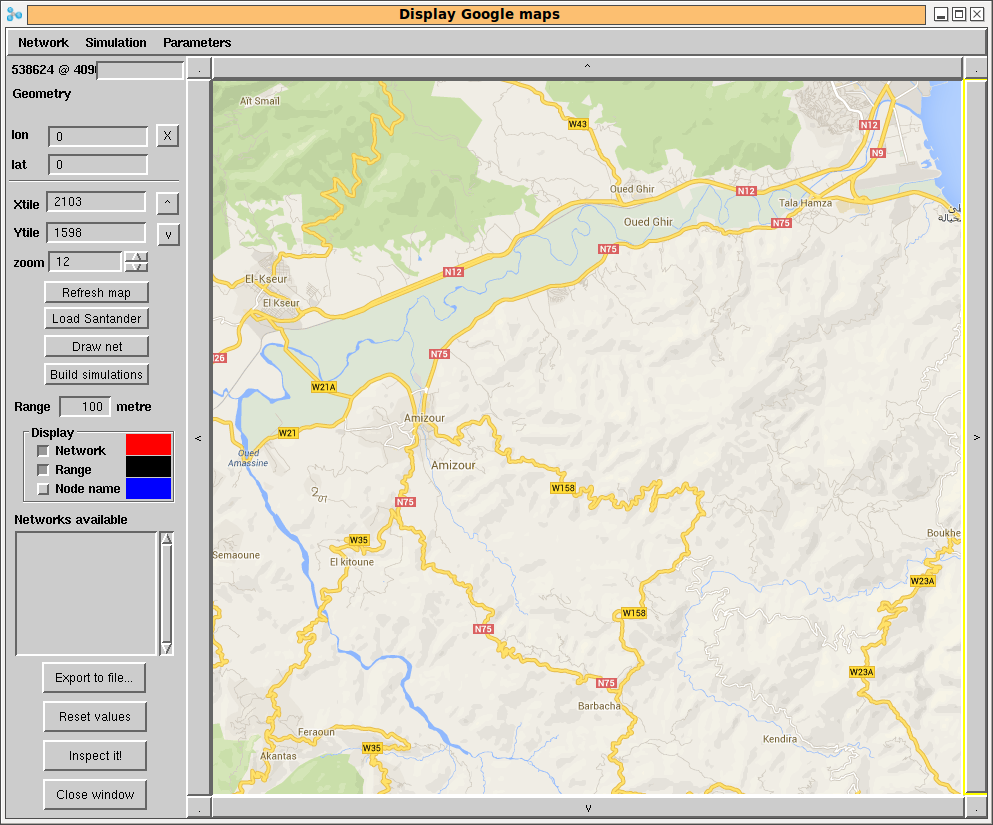
\includegraphics[width=8cm]{soummam0.png}
\caption{The browser is pointing to a North Africa river where sensors are to be installed
for water observations.}
\label{fig:initialSoummam}
\end{center}
\end{figure}


First, let us comments what is a GPX file. In this format, we find a header 
that keep information about the initial source of contents. As an example, 
a header from the Santander website could contain: 

\begin{lstlisting}
<?xml version="1.0" encoding="utf-8"?>
<gpx version="1.0" creator="NetGen for Santander">
  <metadata>
  <name>SmartSantander's sensors</name>
     <desc>Sensors in city: Santander, Spain</desc>
     <link>http://smartsantander.eu/</link>
     <time>2013-06-13T17:45:10</time>
</metadata>
\end{lstlisting}

After this there is a list of entries for each of the location documented by the file. 
In the case of our river, we will find tens of similar entries such as: 

\begin{lstlisting}
<wpt lat="36.679926936710501" lon="4.911090436802451">
  <name>H1-2</name>
  <sym>El Kseur</sym>
</wpt>
<wpt lat="36.682937769536323" lon="4.919011088180600">
  <name>I2</name>
  <sym>El Kseur</sym>
</wpt>
<wpt lat="36.686345105073165" lon="4.929854203839318">
  <name>J3</name>
  <sym>El Kseur</sym>
</wpt>
...
\end{lstlisting}

This a very short information since no practical values appear from sensors. 
The file extraction presents three waypoints (from the initial purpose of the NMEA standard for
GPS), with geographic coordinates as decimal expression of degrees. 
Following we find a name for this particular point, and a symbol to display. 

\subsection{Loading a network}

By using the \emph{Network} menu at top-left we can select the 
\emph{Load Gpx} function that brings a dialog 
to select a GPX file. In our case, it is \emph{soummam.gpx} 
file to remember the name of the river and the file format. 
The file is parsed and its contents appears as points on the graphic part.

The symbols appearing in the entries of the file are used to group waypoints together 
inside networks. This networks are shown in a list in the left column. 
They are selectable, and as an example, the network \emph{El Kseur} is validated 
for display figure \ref{fig:soummam1}. 

\begin{figure}
\begin{center}
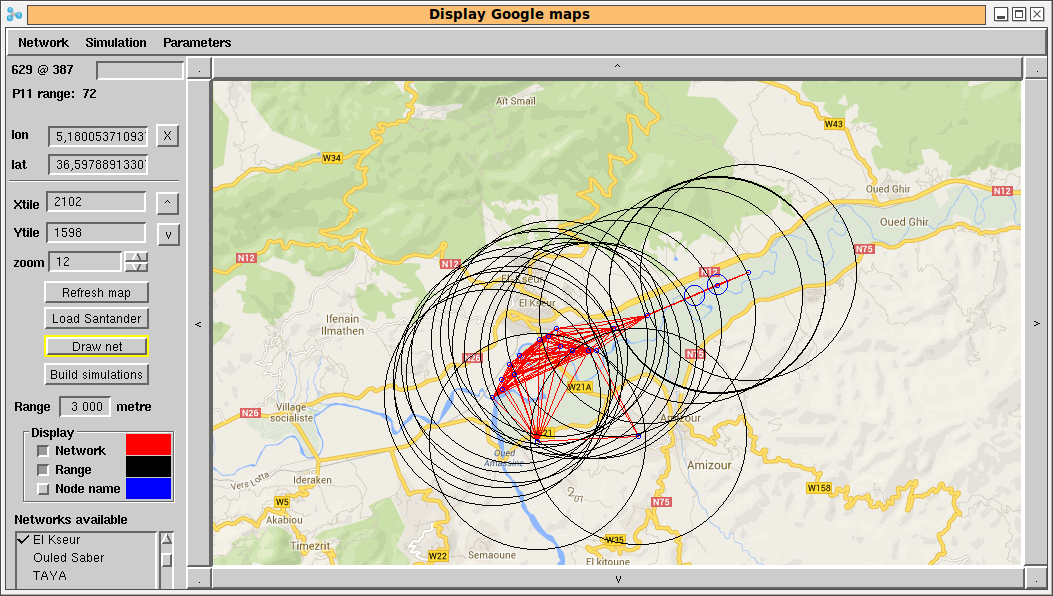
\includegraphics[width=8cm]{soummam1.png}
\caption{The browser is pointing to a North Africa river where sensors are to be installed
for water observations.}
\label{fig:soummam1}
\end{center}
\end{figure}

\subsection{Network configuration}

Several of the functions of NetGen as described in the previous chapter are avalaible from 
this front-end window which capabilities exceed the picking tool shown 
chapter \ref{sec:chapter2}. As an example, the range used to decide wether a sensor 
is connected to another can be defined using a dedicated numeric field. Furthermore, 
the present tool has precise knowledge about geographical points and related distances 
including display distances. Thus, the distance can be defined as meters conforming to 
radio capability specification. 

On figure \ref{fig:soummam1}, the range has been tuned to the point where each sensor 
in the El Kseur network was reachable, giving a necessary range of 3~000 meters to include 
all the sensors. The window does not react directly to range modification, 
it is necessary to call \emph{Draw net} button. 

Some colouring functions ease the display of sensor names, range circles, and connectivities. 

The mouse location over a graphic presentation is tracked on the top-left 
of the window: 

\begin{itemize}
\item point coordinates inside the window, changing to red when the mouse is precisely over 
  a sensor. 
\item this case the logical name of the node is shown in the edit field.
\item a second line presents the range and position of the closest sensor, 
or a communication channel in the case where the mouse is over such a channel.
\end{itemize}


\subsection{Network generation}

To reach Netgen functionalities related to the process graph specification, 
it is sufficient to depress the build simulations button: the specification is 
loaded in every Netgen window (chapter \ref{sec:chapter2} and figure \ref{fig:soummamNetgen})  
for further use: building simulation, graph drawing (see figure \ref{fig:soummamGraph}), etc... 


\begin{figure}
\begin{center}
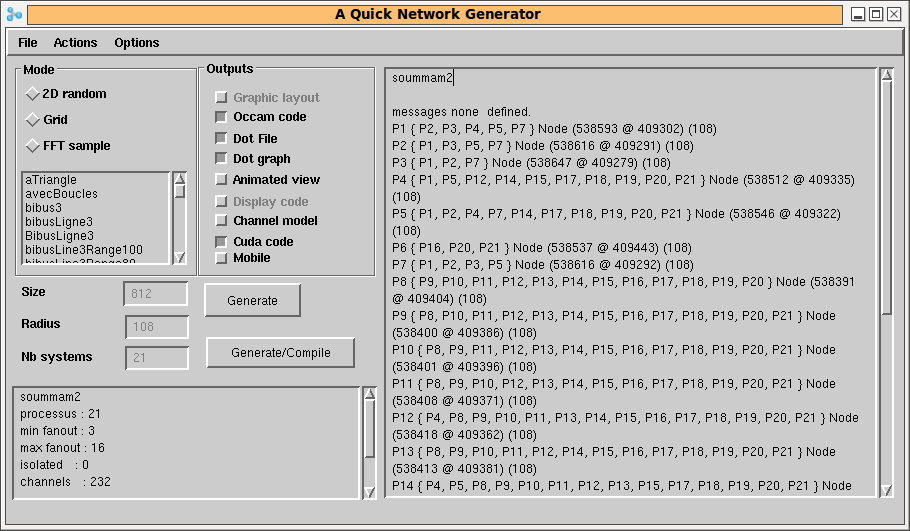
\includegraphics[width=8cm]{netgenSoummam.png}
\caption{Netgen window with El Kseur specification and statistic. }
\label{fig:soummamNetgen}
\end{center}
\end{figure}

\begin{figure}
\begin{center}
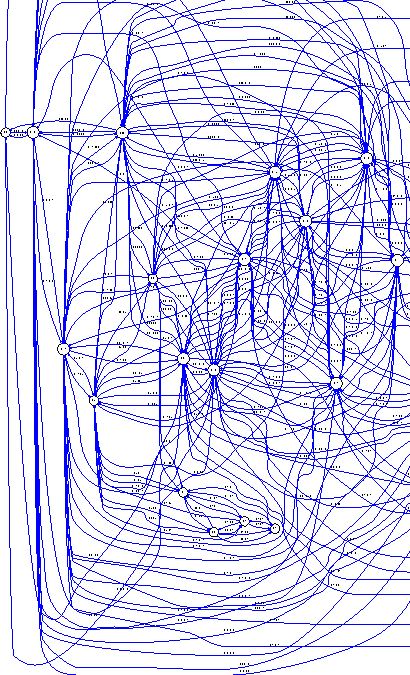
\includegraphics[width=8cm]{soummam2.pdf}
\caption{Logic graph for El Kseur location network.}
\label{fig:soummamGraph}
\end{center}
\end{figure}



After this exploration we have learned that this network has 21 nodes with maximum 
connectivity of 16, with 232 communications channels.

Executing the simulation brings a value of 4 hops for the network diameter. 
We probably have interest to reduce the general range keeping the further nodes to 
a 3~000 m range. 

\section{Loading building architectures}

The package concerned with building representations is MapAccess one, also available from 
the same store server as for chapter \ref{sec:chapter1}. 

In addition to this package, we need some files in the format of "shapefile". This time, 
we propose to do our scenario on the case of Brest city which administration decided 
to produce large description as 80~000 buildings set. 

\begin{itemize}
\item start a fresh image and ensure that the NetGen package is loaded with one of the last
version (1.28.1.2.5 should work)
\item open the store dialog from VisualWorks main window
\item select GoogleMap package (we need to change this name)
\item select version 1.15.5.2 or later, and type load from the pop-up menu

\item
This comment is as follows: 
Display maps from tile servers, like Google Map or OpenStreetMap.
Georeference points on the map.
Display objects from shapefiles. 
Library is located here: http://wsn.univ-brest.fr/MapAccess/library/libShapeFile.tar. Run 'make' to compile it. 
BMO shapefile is located here: http://wsn.univ-brest.fr/MapAccess/bmo/. Copy the two files shp and shx in the same directory. 


\end{itemize}




\chapter{Physical modelling}

Combining physical simulation and sensor network simulation allows to verify
the accurracy of the sensing process in relation with the physical process.
In most of the cases, the two activities are independent, but there are known situations
where a control loop exist.

This chapter will shortly discuss preliminary works where geographic data are
extracted (see chapter \ref{sec:chapter5}), analyzed, and processed to simulate the
the physical process:
\begin{enumerate}
\item case of a mobile moving inside a set of sensors,
\item case of cellular automata representing physical process.
\end{enumerate}


In these situations the physical process spread over 2D or 3D spaces, that are
divided into a number of adjacent cells. One solution to keep track of evolutions 
is to use massive parallelism with a good computation candidate being cellular automata.


\chapter{PickCell: from image analysis to physical simulation} 
 
{\sl The associated software is available in the Pickcell package pn Store at http://wsn.univ-brest.fr.
Use is similar to  chapter  \ref{sec:chapter5bis} explanations: 
\begin{itemize}
\item load pickcell, then load a file image from the application window seleted from Tool menu,
\item load quickmap, then select the quickmap pickcell variant from tool menu, to enable
pickcell from an OpenStreetMap view.
\end{itemize}
}


Creation of sensing machines working in the environment necessitate 
a validation  in the context of physical scenarios. Some of these 
scenario are flooding, insect clouds, pollutions, fires.

The focus of this chapter are tools and methods allowing to produce inputs and  organizations
for physical  simulations. These simulation involve lot of computations. A  choice
is to use  space and time  discrete  models such as
cellular automata. It is also expected that physical simulation  will cooperate with network simulations
in various ways: production of stimuli on sensors, or  modificaton  of the sensor network 
itself. Figure \ref{fig:physics+sensorsFlow} displays the general scenario with
the left branch being discussed here.



\begin{figure}[hbtp]
\begin{center} 
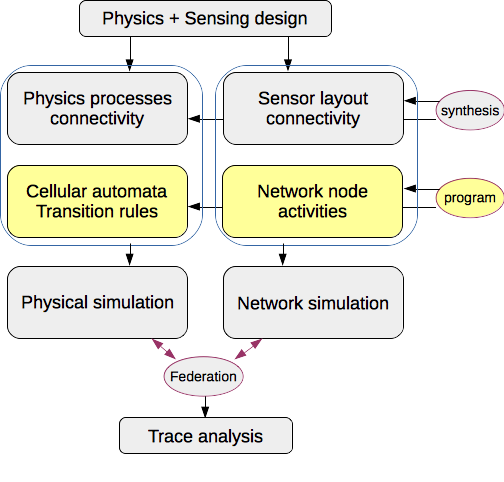
\includegraphics[width=8cm]{physics+sensorsFlow.png}
\caption{General flow for simulation with the physical simulation and the network simulation.
Both share coordination  informations such as geographical or geometrical points, clocking system,
and they can be coordinated during the simulation.}
\label{fig:physics+sensorsFlow}
\end{center}
\end{figure}


The interest of image anlysis is to  produce sets of  regions that share similar characteristics.
Analysis follows a conventional flow, starting from a picture coming  from
photographies, maps, radar images, to obtain regions of interests, on which physical simulation  will
take place.

\begin{figure}[hbtp]
\begin{center} 
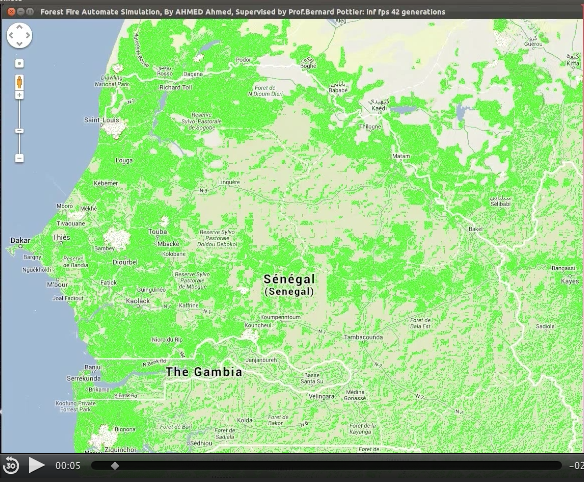
\includegraphics[width=10cm]{AhmedFire.png}
\caption{Example of a fire simulation  using Cellular Automata  cells that have  states such as:
vegetation, burning, ashes.}
\label{fig:AhmedFire}
\end{center}
\end{figure}

A reference for processing on such regions are cellular automata
reproducing fire expansions of phenomenon consuming  vegetation.
Figure \ref{fig:AhmedFire} is extracted from a
movie demonstration where "fires" are started randomly to "eat" such vegetation report \cite{AhmedFire}. This
preliminary work was achieved on an Nvidia GPU.

The chapter will provide details on the production of   systems representing the physical
process working in harmony with the sensing systems.

\section{Image processing  flow for cellular system synthesis}

Thus,   modeling  physical regions automatically, or semi-automatically, following physical process 
characteristics, is certainly critical to lead both physical and control network  simulations jointly,
and synchronously. One can think of this as a sampling technique of the physical process sharing
a clock with the sensing network. Cellular automata are one way to implement the real world simulation,
starting from initial states and regions.


A general flow to obtain such regions  is  shown figure \ref{fig:pickcellFlow}~:
\begin{enumerate}
\item  preprocessing  images 
\item segmenting images into blocks
\item recognition of similar cells and grouping into regions
\item processing regions an obtaining skeleton images
\end{enumerate}

\begin{figure}[hbtp]
\begin{center} 
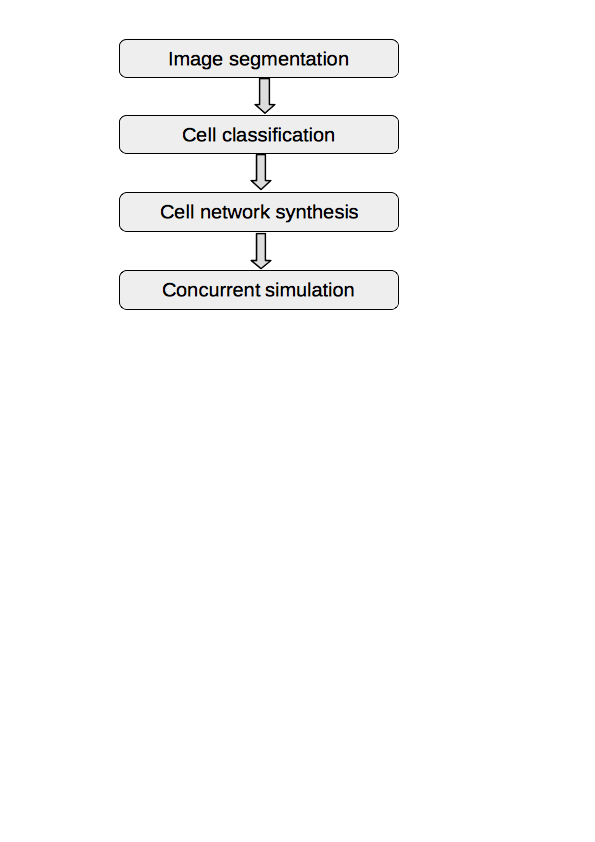
\includegraphics[width=6cm]{pickcellFlow.png}
\caption{Preparing cellular automata from image analysis: synthesis flow.}
\label{fig:pickcellFlow}
\end{center}
\end{figure}

Following this flow, higher level objects can be obtained, still with geographical definition in the case of
maps, or satellite imagery.

\subsection {Preprocessing for image preparation }

In the case of maps, geographic information is yet presented in a comprehensive way. However analyzing maps is still useful
to obtain information without the direct contact of an initial information system (GIS).
More difficult is the case of satellite or air  images, because the synthesis of objects necessitate
pre processing. Figure \ref{fig:sideBySide} shows an example of procesing achieved using common tools
for management of photographies. The initial view is a satellite image (left), while the right part displays an improved
view, with better contrasts.

\begin{figure}[hbtp]
\begin{center} 
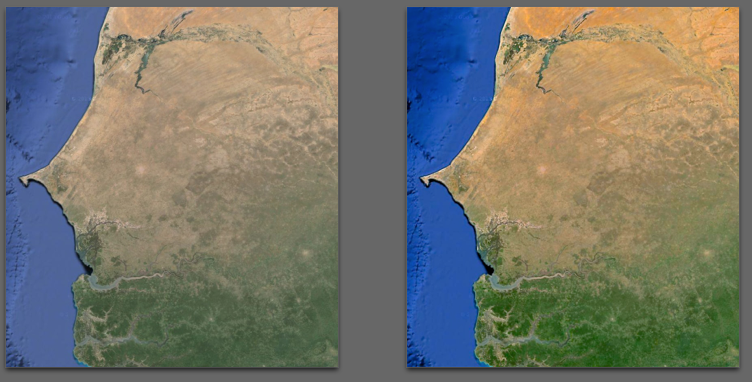
\includegraphics[width=10cm]{SenegalSideBySide.png}
\caption{Modifying original image for better contrasts or coulour selections. Image is a satellite view from Google Maps.}
\label{fig:sideBySide}
\end{center}
\end{figure}

These representations are coming from a very common image processing software 
allowing to change contrasts and colour mapping to fit tne necessity of the recognition.
Image processing paramers show the Red Green Blue statistic values in the original
and the modified image, with a better use of the value range in the second case
(Figure \ref{fig:colours1+2}).



\begin{figure}[hbtp]
\begin{center}
\leavevmode 
\begin{minipage}{6cm}
\begin{center} 
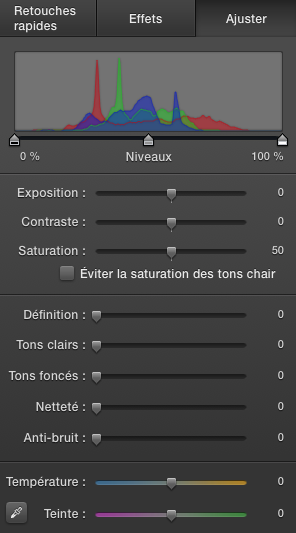
\includegraphics[width=6cm]{senegalColours.png} 
\end{center}
\end{minipage}~~~~~~~~~\begin{minipage}{6cm}
\begin{center} 
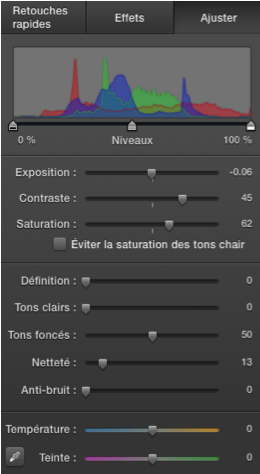
\includegraphics[width=6cm]{senegalColours2.png} 
\end{center}
\end{minipage}
\caption{RGB colour statistics for the left original picture, and its adaptation (right). The software
is Apple iPhoto, standard to any MacOs computer. Similar functions could be obtained from Linux GIMP,
and probably reimplemented from a Palette tool in NetGen.}
\label{fig:colours1+2}
\end{center}
\end{figure}
  
\subsection { Segmenting the image into cells}

To obtain regions, it is necessary to group zones of the image based on similarities of different kind.
The first operation is a fragmentation into blocks of different size and geometry. Of course,
squares, or rectangles are the simplest way to proceed, but other fragmentation techniques could also
be suitable and ease further stages in simulation. Cellular automata propose as example  an hexagonal
shape where each cell has 6 direct neighbours.

{\sc PickCell} has been implemented     to ease this fragmentation, in relation with 
further networks synthesis operations.

This tool reuse the {\sl Picking} framework presented Figure  \ref{fig:PickPoint1}. Beside the capability
to load images, and specify sensor positions, there is the ability to install a rectangular grid over the
image.


\begin{figure}[hbtp]
\begin{center} 
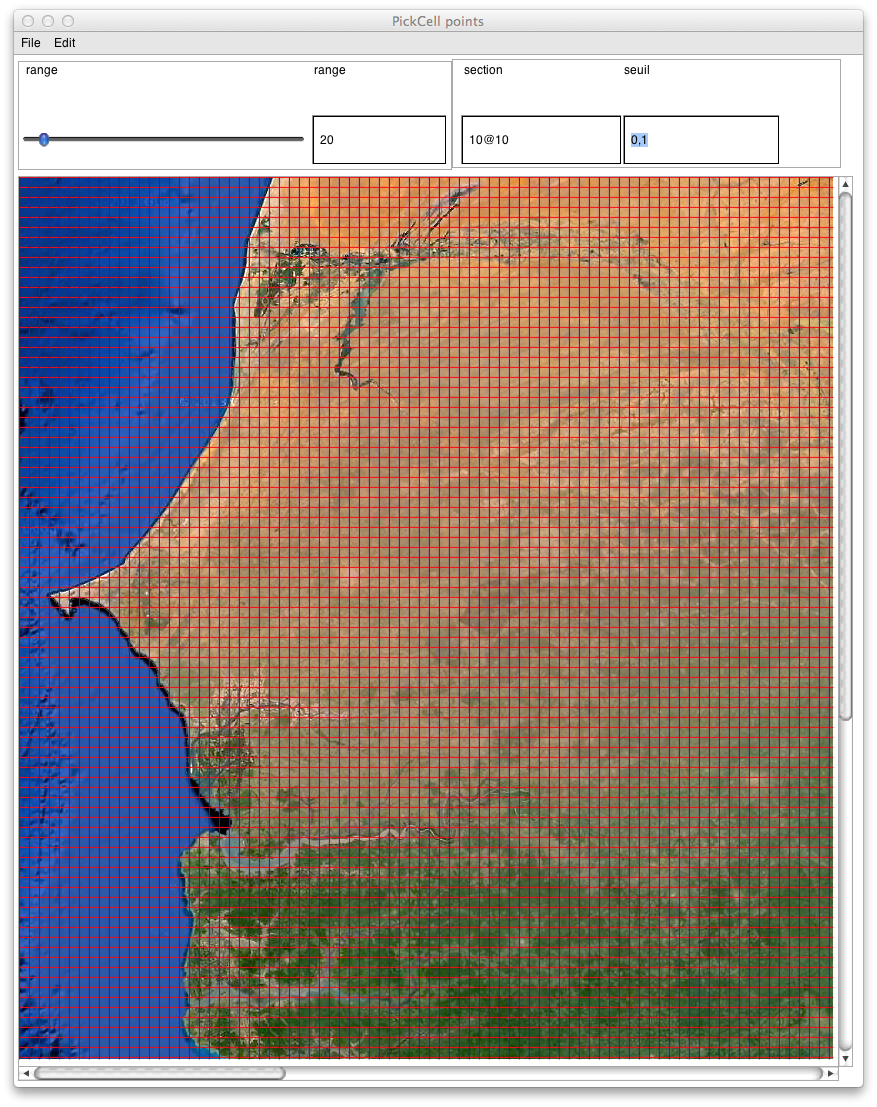
\includegraphics[width=10cm]{SenegalGrid10x10.png}
\caption{Using a 10@10 grid, the image is split into $10\times10$ pixels. 
Following the application, it is possible to specify $x  \times   y$ grids with $x  \neq  y$.}
\label{fig:SenegalGrid10x10}
\end{center}
\end{figure}

Having split the image into cells, it is now possible to classify thems around common properties.

\begin{figure}[hbtp]
\begin{center} 
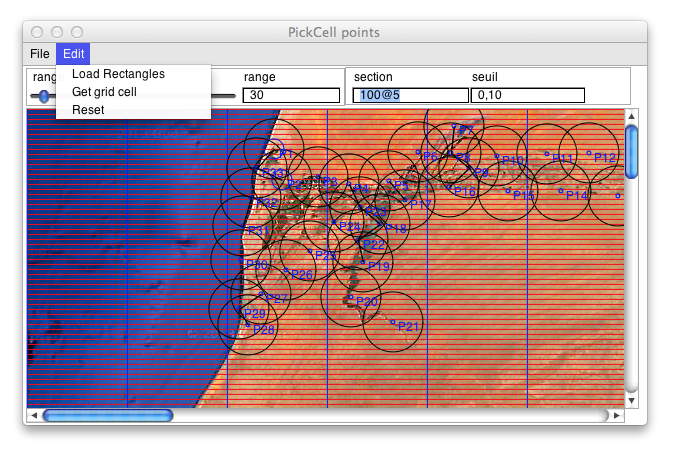
\includegraphics[width=10cm]{SenegalGetGridCell.png}
\caption{Rectangular grid, and sensor geometry specification. The Edit Menu {\sl Get Grid Cell} allows to go a step forward in the flow
to group cell togethers and form {\sl regions} of interest. Section \ref{sec:classification}}
\label{fig:SenegalGetGridCell}
\end{center}
\end{figure}

\subsection { Grouping cells  into classes}
\label{sec:classification} 
\subsubsection { Computing statistics}

From the menu shown Figure  \ref{fig:SenegalGetGridCell}, we obtain a new tool for region
specification and manipulation. As for the grid in segmentation, a new parameter allows to divide
the cell space according to pixel distributions.The choice of group distribution  can be more or less sophisticated.
To start by the begining, the following algorithm is applied to the whole cell grid, to obtain a set of $min, max, mean$ parameters
on each colour :

\begin{lstlisting}  
STEP 1
	for each cell in the grid
		for each pixel in the cell 
			 for each colour component in { R, G, B}
				 update (min(colour))
				 update (max(colour))
				 update (sum(colour))
		 for each colour component in { R, G, B}
			 update (mean(colour))
\end{lstlisting}

Following this step, we have $3 \times 3$ parameters set in each cell, thus allowing to compute
global image characteristics that will reflect the efficiency of the preprocessing:

\begin{lstlisting}  
STEP 2
	for each cell in the grid
		for each colour component in { R, G, B}
			update(minGlobal)
			update(maxGlobal)
			update(minMeanGlobal)
			update(maxMeanGlobal)
\end{lstlisting}


\begin{figure}[hbtp]
\begin{center} 
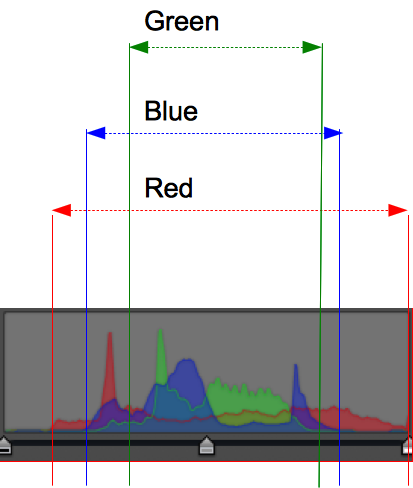
\includegraphics[width=6cm]{RGBDiagram.png}
\caption{From the preprocessing results shown Figure \ref,{fig:colours1+2},   we can guess min(colour), max(colour) for each
component in Red Green Blue.}
\label{fig:RGBDiagram}
\end{center}
\end{figure}

After this step and for each component in RGB space, we have global $[min,max] $ measures for:

\begin{itemize}
\item the value taken over the image (see Figure \ref{fig:RGBDiagram} )
\item the mean of values in each cell
\end{itemize}



\subsubsection { Grouping cell together }

We can use the values computed in each cell and globally to group cell togethers. For the minimum
and the maximum, and even the mean in each cell, a simple algorithm is as follows:

\begin{lstlisting}  
STEP3
	decide on a partition in N>1
	for each component in RGB
		discard any value out side the  [min,max]   interval found for the component
		produce N adjacent sub intervals   [min,max]  
\end{lstlisting}

In the case of $N=2$ the RGB min, max, or mean values in each cell will allow to {\sl classify}
each cell in an unique way in a $2^3$ interval space $(R_0,R_1) \times (G_0,G_1) \times (B_0,B_1) $.
The {\sl cube} of coordinates go from $0,0,0= 0$ to $1,1,1= 7$.
By selecting {\sl Get grid cell} shown Figure \ref{fig:SenegalGetGridCell} the classification tool appears.

What does this too is to allow the selection of $N$, then each cell is tne image is assigned to an interval
depending on its values. By selecting codes as defined above, the corresponding regions appear
an part of the original image. 


\begin{lstlisting}  
STEP4
	for each interval allocate a collection to record cells pertaining to this interval
	for each cell in the grid record the cell in its interval with the geographic position
\end{lstlisting}


\begin{figure}[hbtp]
\begin{center} 
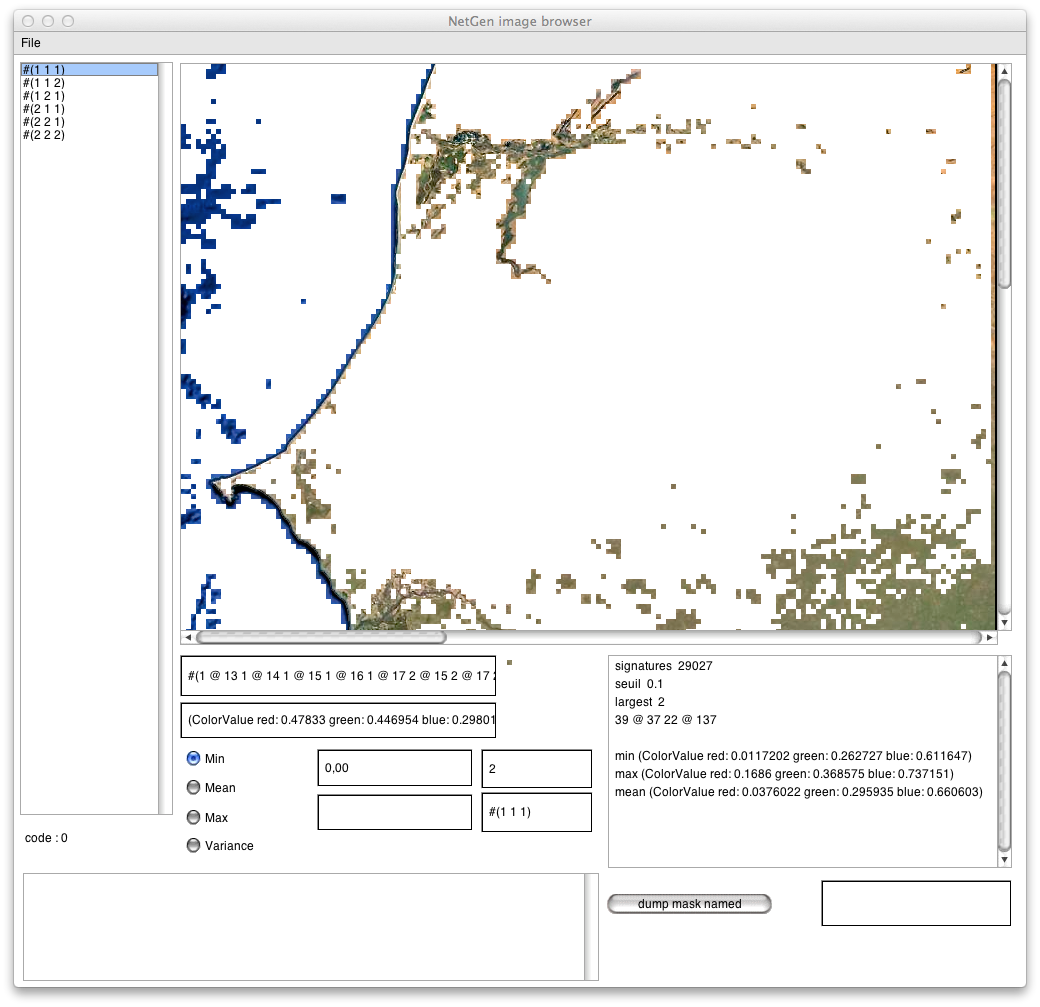
\includegraphics[width=12cm]{Senegal5x5code0.png}
\caption{Pixel class  browser displaying the region corresponding to code 0 : lowes interval in each component of R, G, B.
Shore and rivers appear as dark cell when the minimum criteria are selected. The partition is N=2, code is 0, for (R=1,G=1,B=1).}
\label{fig:Senegal5x5code0}
\end{center}
\end{figure}

\section{Cell system synthesis}
\subsection { Weaving a  network }

Given a cell system produced from a class, grouping several classes, or from a whole image, 
we can now consider to produce a process organization. Taking one node, there are many way to decide
which neighbours are visible, and this task can appear simple if we use a connexion pattern.
Cellular automata use these patterns to define neighborhood.

Examples of neighborhood are Von Neumann cross, or Moore square. Mathematical morphology
methods allow these neighborhood to be arbitrary shapes. As an example two line segments
could figure a plane in the sky.


\begin{figure}[hbtp]
\begin{center} 
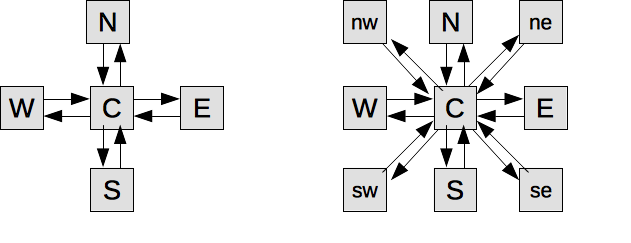
\includegraphics[width=10cm]   {VonNeumann.png}
\caption{Von Neumann and Moore neigborhood with distance = 1}
\label{fig:VonNeumann}
\end{center}
\end{figure}

To build a cell system, the class is swept, row by row, column by column.
For each existing cell, a process is created.

In a second stage,   the class is again swept cell by cell.
For each cell C,   the neighborhood positions  are searched   inside the class.
For each existing neighbour, links are established with the center C.
This way a network of celles is weaved according to the neighborhood
and the class geometric organization. Figure \ref{fig:classBrowser}
displays the Cell class browser with choice of standard neighborhhod at the bottom.




\begin{figure}[hbtp]
\begin{center} 
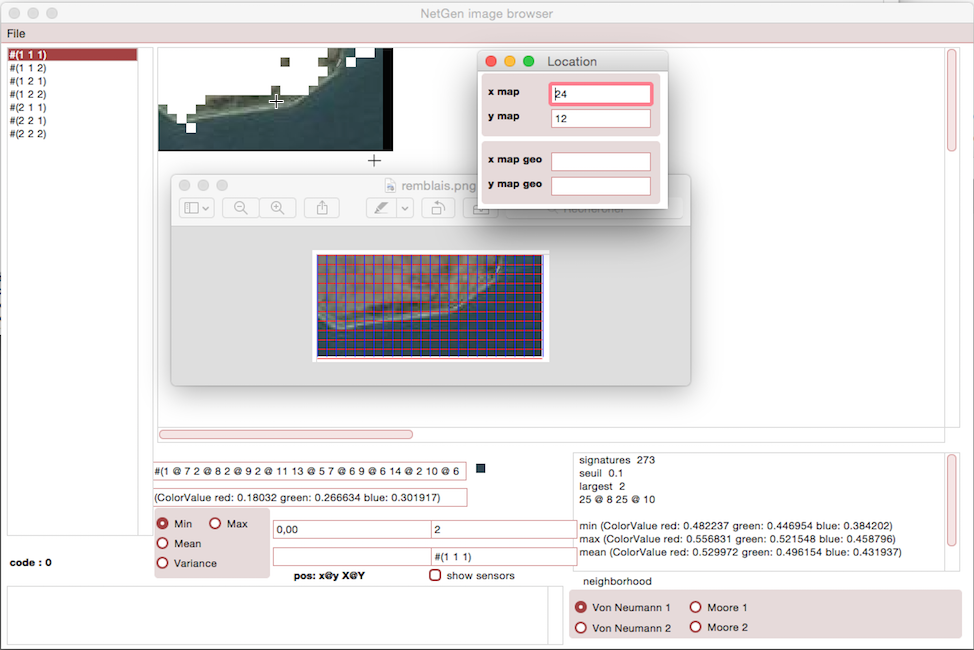
\includegraphics[width=12cm]{classBrows+Loc+mask.png}
\caption{Segmented image and its distribution into classes, code 0 selected.
Picture shows a cross cursor above one of the cell ant the location of the cell.
This cell has neighbours at North, South, East and West, and thus has a full Von Neumann neighborhood.
However a Moore neighborhood would be incomplete due to cells lacking in the north}
\label{fig:classBrowser}
\end{center}
\end{figure}

\begin{figure}[hbtp]
\begin{center} 
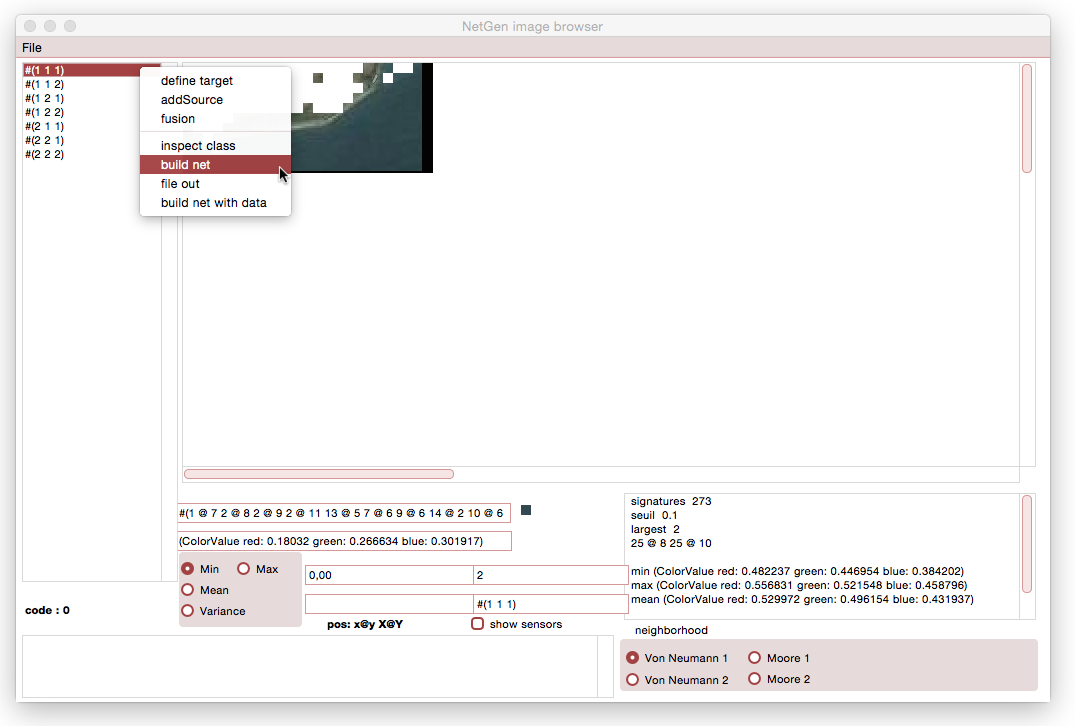
\includegraphics[width=8cm]{generatingCellNetwork.png}
\caption{Calling the network generator on a cell class}
\label{fig:generatingCellNetwork}
\end{center}
\end{figure}
\subsection {Programs generation }

Once the network is built, programs can be produced to represent its process and topology.
Menu in the cell class list has a {\sl Build net} option for this (figure \ref{fig:generatingCellNetwork}.
The results are produced in NetGen windows available as shown figure  \ref{fig:cellNetworkSample}.
There is atmost 4 processes in the fanout for each cell, and isolated process are removed.
The abstract network is described as shown below~:
\begin{lstlisting}
cellNetwork0

messages none  defined. 
Px23y8 { Px22y8, Px23y9, Px24y8, Px23y7 } CellNode (23 @ 8) (20)
Px20y10 { Px20y9, Px20y11, Px21y10, Px19y10 } CellNode (20 @ 10) (20)
Px17y7 { Px17y6, Px16y7, Px17y8, Px18y7 } CellNode (17 @ 7) (20)
Px12y8 { Px12y9, Px12y7, Px13y8, Px11y8 } CellNode (12 @ 8) (20)
...
\end{lstlisting}


In this text, each process is named using its position, as example $Px23y8$ is located at
row 8, columns 23. The name of the procedure executed is CellNode() to distinguish with Node()
used inside sensor networks. Positions and range also appear at the end of the line.


\begin{figure}[hbtp]
\begin{center} 
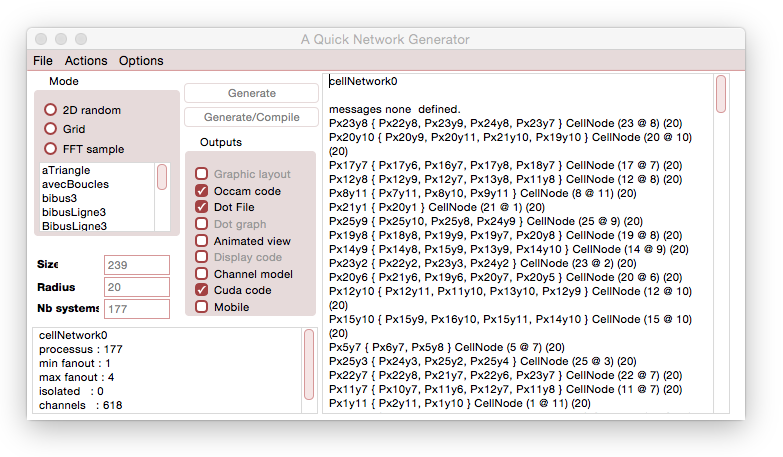
\includegraphics[width=12cm]{cellNetworkSample.png}
\caption{Screencast showing the abstract specification of a generated network for code 0 class.
One process per line, as for sensor networks.}
\label{fig:cellNetworkSample}
\end{center}
\end{figure}

Statistics show that fanout is limited to four, fanin at least equal to 1. There are 177 cells.
Occam (and CUDA) process systems have been produced by the generator that  still need
behaviour description for  their  cella. This behaviour can be very standard transition rule
for cellular automata, but networking behaviuor could apply as well:

\begin{itemize}
\item diameter computation : longest distance between cells,
\item leaders : for naming and differentiating subnetworks
\item routing tables : to reach any cell from any cell in the same network
\item packet transport and delivery, etc\ldots
\end{itemize}

\subsection {Compiling and simulating }

The shortest path to simulate is to reuse a sensor network Occam behaviour file,
as example for leader and diameter dynamic computation. The Actions menu
of NetGen window allows to do it (figure \ref{fig:NetGenAlgo}).

\begin{figure}[hbtp]
\begin{center} 
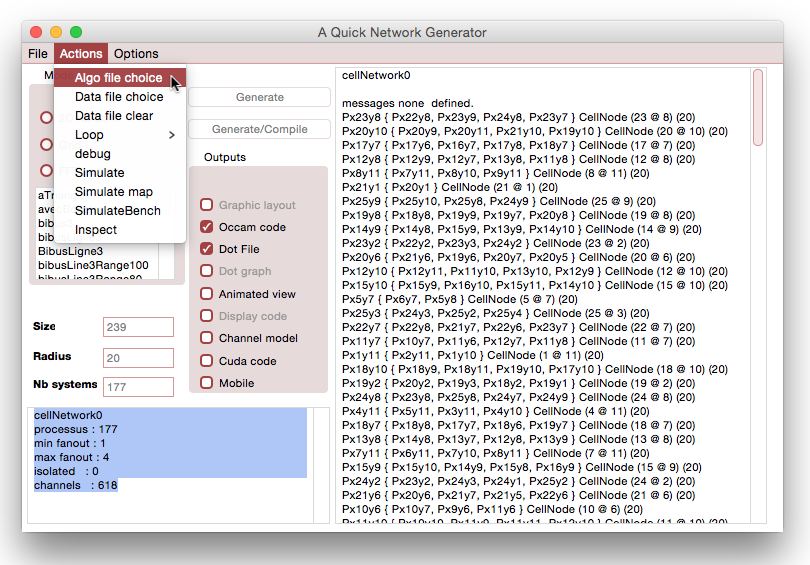
\includegraphics[width=12cm]{NetGenAlgoFile.png}
\caption{Selection of include files: for  behaviour, and also for data files holding the cell contents.}
\label{fig:NetGenAlgo}
\label{fig:includeFiles}
\end{center}
\end{figure}

Once this is done, the action flow is asfollow:
\begin{enumerate}
\item Check coherency between behaviour file and architecture file: in particular the name of the
procedures executed by processes must be the same. For this example, it is CellNode(),
defined in {\sl cellnodes-test-include-diam.occ}.
\item Compile architecture. As example :\\
kroc -lcourse cellNetwork17.occ
\item Check the execution trace.
\end{enumerate}


\section {Physical cell system illustration :  Antsiranana geography capture and analysis }

\begin{figure}[hbtp]
\begin{center} 
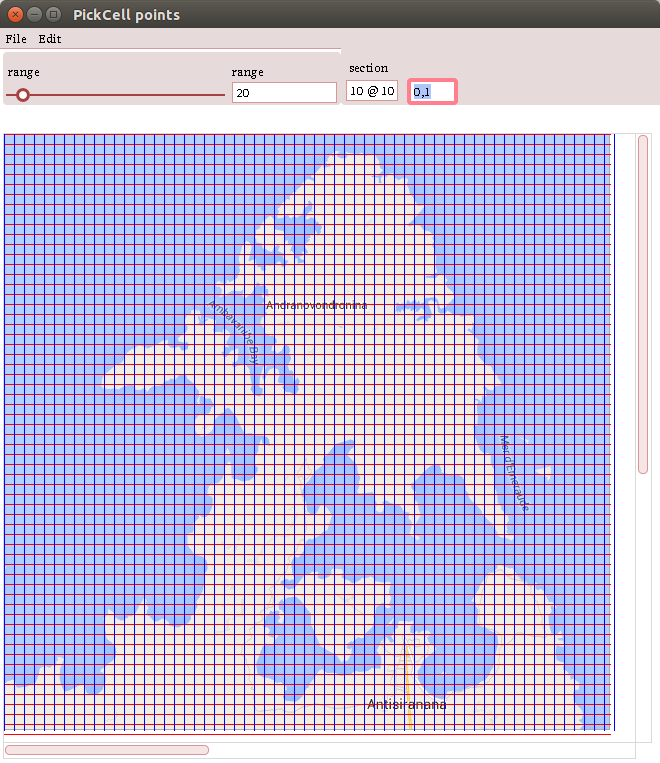
\includegraphics[width=10cm]{diego-split-10x10.png}
\caption{Google map API3 was used to select Antsiranana bay and feed PickCell : $10 \times 10$ pixel cells.}
\label{fif:sampleAntsiranana}
\end{center}
\end{figure}

\subsection {Sample : Antsiranana  cell classification  }

We then select one pixel space and generate networks. and graph for neighborhood VonNeumann 1
The graph seems to present a single network, isn't it?

\begin{figure}[hbtp]
\begin{center} 
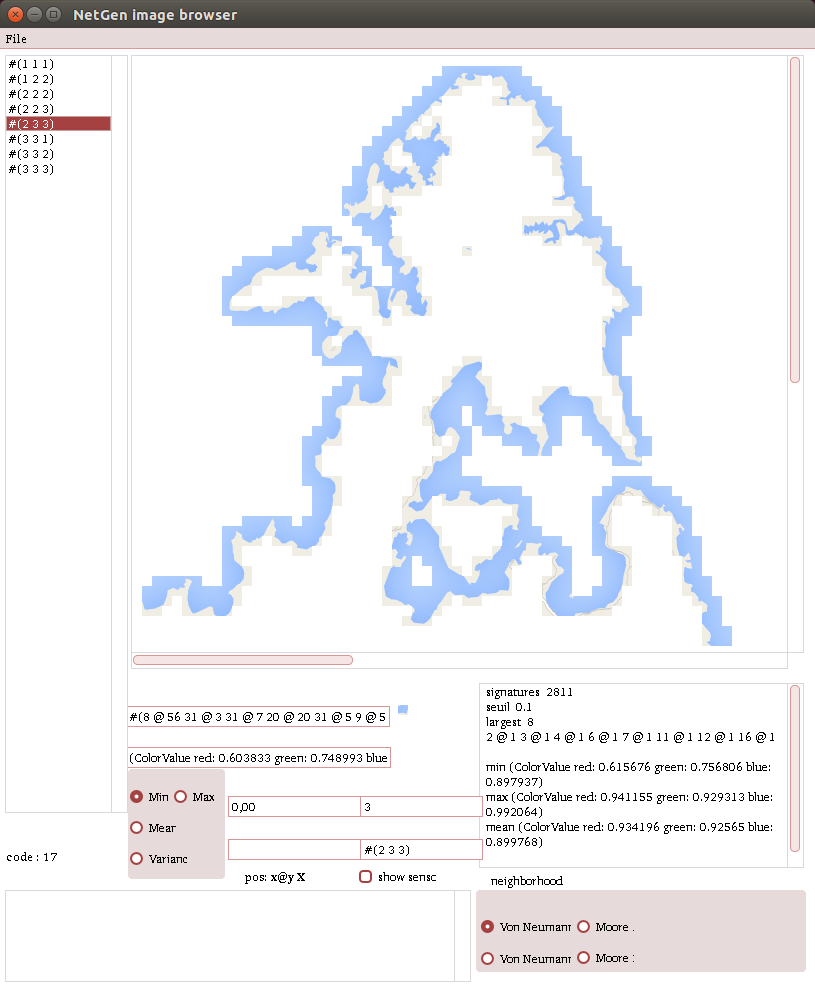
\includegraphics[width=10cm]{diego-class17-3.png}
\caption{The pixel  space was split into 27 subspaces  defining classes.}
\label{fig:antisrananaClass17}
\end{center}
\end{figure}


\begin{figure}[hbtp]
\begin{center} 
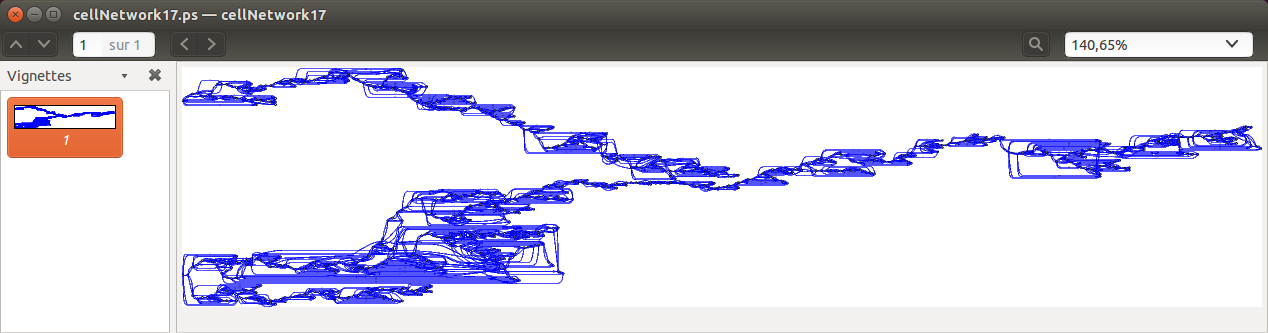
\includegraphics[width=12cm]{diegoGraph17.png}
\caption{Resulting   logic  graph for Von Neumann1 neighborhod.  How many subgraphs  ? see section \ref{sec:comment} }
\label{fig:ansirananaGraph}
\end{center}
\end{figure}

\subsection{ Neighborhood statistics}

The four standatd neighborhood were selected in turns. Statistics came from the NetGen window
after accepting the different network (table \ref{tab:uneCATable}).


\begin{table}[htb]
\begin{center}
\begin{tabular}{|l|l|l|l|l||}\hline
cellNetwork17 & VN1 &   VN2 &   M1 &    M2\\\hline
processus  &    809 &   809 &   809 &   809\\\hline
min fanout  &   1 &     3 &     2 &     6\\\hline
max fanout  &   4 &     12 &    8 &     22\\\hline
isolated    &   0 &     0 &     0 &     0\\\hline
channels    &   2440 &  6346 &  4576 &  10962\\\hline
neighborhood size  &   4 &  12 &  8 &  22\\\hline
\end{tabular}
\caption{ Four different neighborhood generated for Antsiranana bay with distances 1 and 2.
the table show  cell  networks characteristics. }
\label{tab:uneCATable}
\end{center}
\end{table}


\subsection{ Trace and execution }
\label{sec:antsiranan}

Once the program is compiled, we can launch an execution, with more than 800 processes
working together. The program compute the leader Id, and the diameter of network(s).
The trace coming from execution has the following contents:


\begin{lstlisting}
 Id	diam	leader
 784	  84 803
   2	  84 803
   5	  84 803
...
 803	  84 803
 668	 197 808
   0	 197 808
   1	 197 808
...
\end{lstlisting}

\begin{table}[htb]
\begin{center}
\begin{tabular}{|l|l|l|}\hline
identity  & diameter  & leader \\\hline
 784&	  84& 803\\\hline
   2	&  84 &803\\\hline
   5	&  84 &803\\\hline
... & .. & ..\\\hline
 803&	  84& 803\\\hline
 668&	 197& 808\\\hline
   0	& 197& 808\\\hline
   1	& 197& 808\\\hline
... & .. & ..\\\hline
 806	& 197& 808\\\hline
 807	& 197& 808\\\hline
 808	& 197& 808\\\hline
\end{tabular}
\caption{Simulation trace: smallest networks (84-803)  finish first in the case of Occam execution.
It is not the case for CUDA execution. }
\label{tab:uneTableTrace}
\end{center}
\end{table}

Therefore we have two {\sl cell networks } of leaders 803 and 808, and diameters 84 and 197.
Any information circulating in the second network will use at most 197 hops to
reach a destination.

All the algorithms  are not equivalent. See table \ref{tab:uneTableBench} showing a comparison between A and 
running on a multicore i7 CPU. It is noticeable that B has a strong advantage and a higher level
of effective parallelism (see the user row).

\begin{table}[htb]
\begin{center}
\begin{tabular}{|l|l|l|}\hline 
time &  A & B \\\hline
real &  5m24.271s &     0m9.843s\\\hline
user &  5m40.865s &     0m28.074s\\\hline
sys  &  0m0.686s  &     0m0.674s\\\hline
\end{tabular}
\caption{ Two programs A and B executed on the same network. A is for naive
leader and diameter computations. B is for diameter computation saving useless
data transmission. }
\label{tab:uneTableBench}
\end{center}
\end{table}

\section{Neighborhood discovery and isotropy}

As for computer networks,  cellular automata built from analysis have irregularities:

\begin{itemize}
\item shape are  produced from classes, and shapes have frontiers. That means that
if a Von Neumann neighborhood was taken as a connectivity pattern, cells do not have
complete neighborhood.
\item another problem comes from this lack of completion: how can we guess the direction addressed
by a link array ? Which link lead to where ?
\begin{itemize}
\item in the physical world links do not really exist, but direction can be significant,
\item cellular automata can be isotropic, or anisotropic, making directions critical
in transition rules.
\end{itemize}
\end{itemize}




Figure \ref{fig:antisrananaClass17} display a shore obtained from a map system.
As discussed in section \ref{sec:antsiranan} the cell network is distributed into
two parts showing diameters as large as 197 cell paths. If we are to model the effect
of a particular wind on surface tides, we need to know the direction available at each
cell point.

Thus local connectivity discovery is needed. As for sensor networks, it is interesting
to maintain connectivity knowledge  dynamically, and thus, during simulation.

 \subsection {Neighbourhood data structures explained }

The element of Occam coding below allows to see what will append. Basically there
is a descriptor for each detected neighbour. These descriptors will be stored
in a dynamic table, and a redefinition of link protocol allows to pass these tokens
on communication links (abstract, of course).

\begin{lstlisting}  
DATA TYPE KnownNeighbour
  RECORD
    INT Id: -- node identity
    INT linkIndex:  -- index of link
    Location relativeLoc: -- xLoc yLoc record
:
DATA TYPE Neighbourhood
  RECORD
    INT limit: -- to manage table size
    [MaxFanOut] KnownNeighbour knownNeighbour:
:
PROTOCOL diam.proto
  CASE
    null; BYTE
    file; FileOfId
    int; INT
    location; KnownNeighbour -- for neighbour discovery
:
\end{lstlisting}



Initially each cell has its Id and absolute location stored in a KnownNeighbour
record. The problem is to fill the Neighbourhood table with elements coming
from connected cells.



 \subsection {Neighbourhood   discovery }

In our synchronous simulation frame work, this is a single exchange step
followed by the local building of the neighbourhood table.


\begin{lstlisting}
PROC GetNeighbourhood()
  KnownNeighbour me:
  [MaxFanOut] KnownNeighbour them: 
  SEQ
    GetLocation() -- into Location variable loc
    me[Id] := Id  -- Cell Identity
    me[linkIndex] := -1 
    me[relativeLoc] := loc -- absolute location
    PAR
      PAR j=0 FOR SIZE inChan
        inChan[j] ? CASE
          location ; them[j]   -- get tokens from neighbours
            SKIP 
      PAR j=0 FOR SIZE outChan
        outChan[j] ! location ; me -- send our token
    ResetNeighbourhood(myNeighbours)
    SEQ i=0 FOR SIZE inChan
      SEQ
        them[i][linkIndex] := i --recall link index
        AddInNeighbourhood(loc, them[i],myNeighbours)
         -- add a neighbour and translate absolute to relative location
    DumpNeighbourhood(me, myNeighbours, toMux)  -- trace
:
\end{lstlisting}

\subsection {Trace and comment }

This code was added to previous sample, and few lines were extracted.
During the discovery phasis, each node report its identity, its position, then 
the neighborhood table.

The elements extracted all refers to node 482  located at $x= 32, y=53$.
This node has a full VN1 neighborhood with cardinal directions $ N, E, S,  W$
mapped to link $ 3 , 1, 0, 2$. North is relative coordinates $(0,1)$, West is $(-1, 0)$.
The coordinate system see the origin in $(0,0)$ being at top left of an image.

The name of this cell is Px32y53, and its network diameter is 197.
Notice that cell of Id 479 has an incomplete neighbourhood reduced to 3 cells.

\begin{lstlisting}
./cellNetwork17 | grep 482
248 32 54 { 3 0; 0, 1}{ 57 1; 1, 0}{ 245 2; -1, 0}{ 482 3; 0, -1}
306 33 53 { 57 0; 0, 1}{ 380 1; 0, -1}{ 482 2; -1, 0}{ 741 3; 1, 0}
479 31 53 { 245 0; 0, 1}{ 482 1; 1, 0}{ 564 2; 0, -1}
482 32 53 { 248 0; 0, 1}{ 306 1; 1, 0}{ 479 2; -1, 0}{ 575 3; 0, -1}
575 32 52 { 380 0; 1, 0}{ 482 1; 0, 1}{ 564 2; -1, 0}{ 580 3; 0, -1}
482 Px32y53:
482  197
\end{lstlisting}

We can interpret the trace according to table \ref{tab:cardialAndIndex}. and \label{tab:cardialAndIndex479}.
\begin{table}[htb]
\begin{center}
\begin{tabular}{|l|l|l|}\hline
direction & vector & link index \\\hline
N  &  ( 0, -1) &   3 \\\hline
W  &   ( -1 ,  0 ) &   2  \\\hline
S  &  ( 0, 1) & 0   \\\hline
E  &  ( 1, 0 ) &   1 \\\hline
\end{tabular}
\caption{Node 482 relations between link index and cardinal directions. }
\label{tab:cardialAndIndex}
\end{center}
\end{table}


\begin{table}[htb]
\begin{center}
\begin{tabular}{|l|l|l|}\hline
direction & vector & link index \\\hline
N  &  ( 0, -1) &   2 \\\hline 
S  &  ( 0, 1) & 0   \\\hline
E  &  ( 1, 0 ) &   1 \\\hline
\end{tabular}
\caption{Node 479 relations between link index and cardinal directions. Uncomplete VN1 neighbourhood. }
\label{tab:cardialAndIndex479}
\end{center}
\end{table}




\section { Accessing cell data}

How we can obtain access to cell data produced during image analysis. Look inside
the data file produced as shown figure s \ref{fig:NetGenAlgo} and \ref{fig:generatingCellNetwork}.

\subsection {Data structures }

The data structure appearing in top of the data file are as follows:
\begin{lstlisting}
DATA TYPE ImageExtent -- cell dimension
  RECORD
    INT width:
    INT height:
:
DATA TYPE CellPosition
  RECORD
    INT x:
    INT y:
:
DATA TYPE RGBPixel -- RGB pixel
  RECORD
    BYTE red, green, blue:
:
-- generated description of one cell, size hard coded
DATA TYPE Depth24ByteArray  IS [ 100] RGBPixel:
-- this is a cell image contents with dimensions and contents
DATA TYPE CellImage
  RECORD
    ImageExtent  extent:
    Depth24ByteArray pixelArray:
:
-- this is a complete cell, with its position and data
DATA TYPE CellArray
  RECORD
    CellPosition position:
    CellImage image:
:
-- this is data for one class, 810 cells for this one
VAL [   810] CellArray  Cells IS  -- follows a table of cell contents
-- pages of values
\end{lstlisting}


\subsection {From cell data to cellular automata local state }

(to be continued)






\section { Comments}

\begin{figure}[hbtp]
\begin{center} 
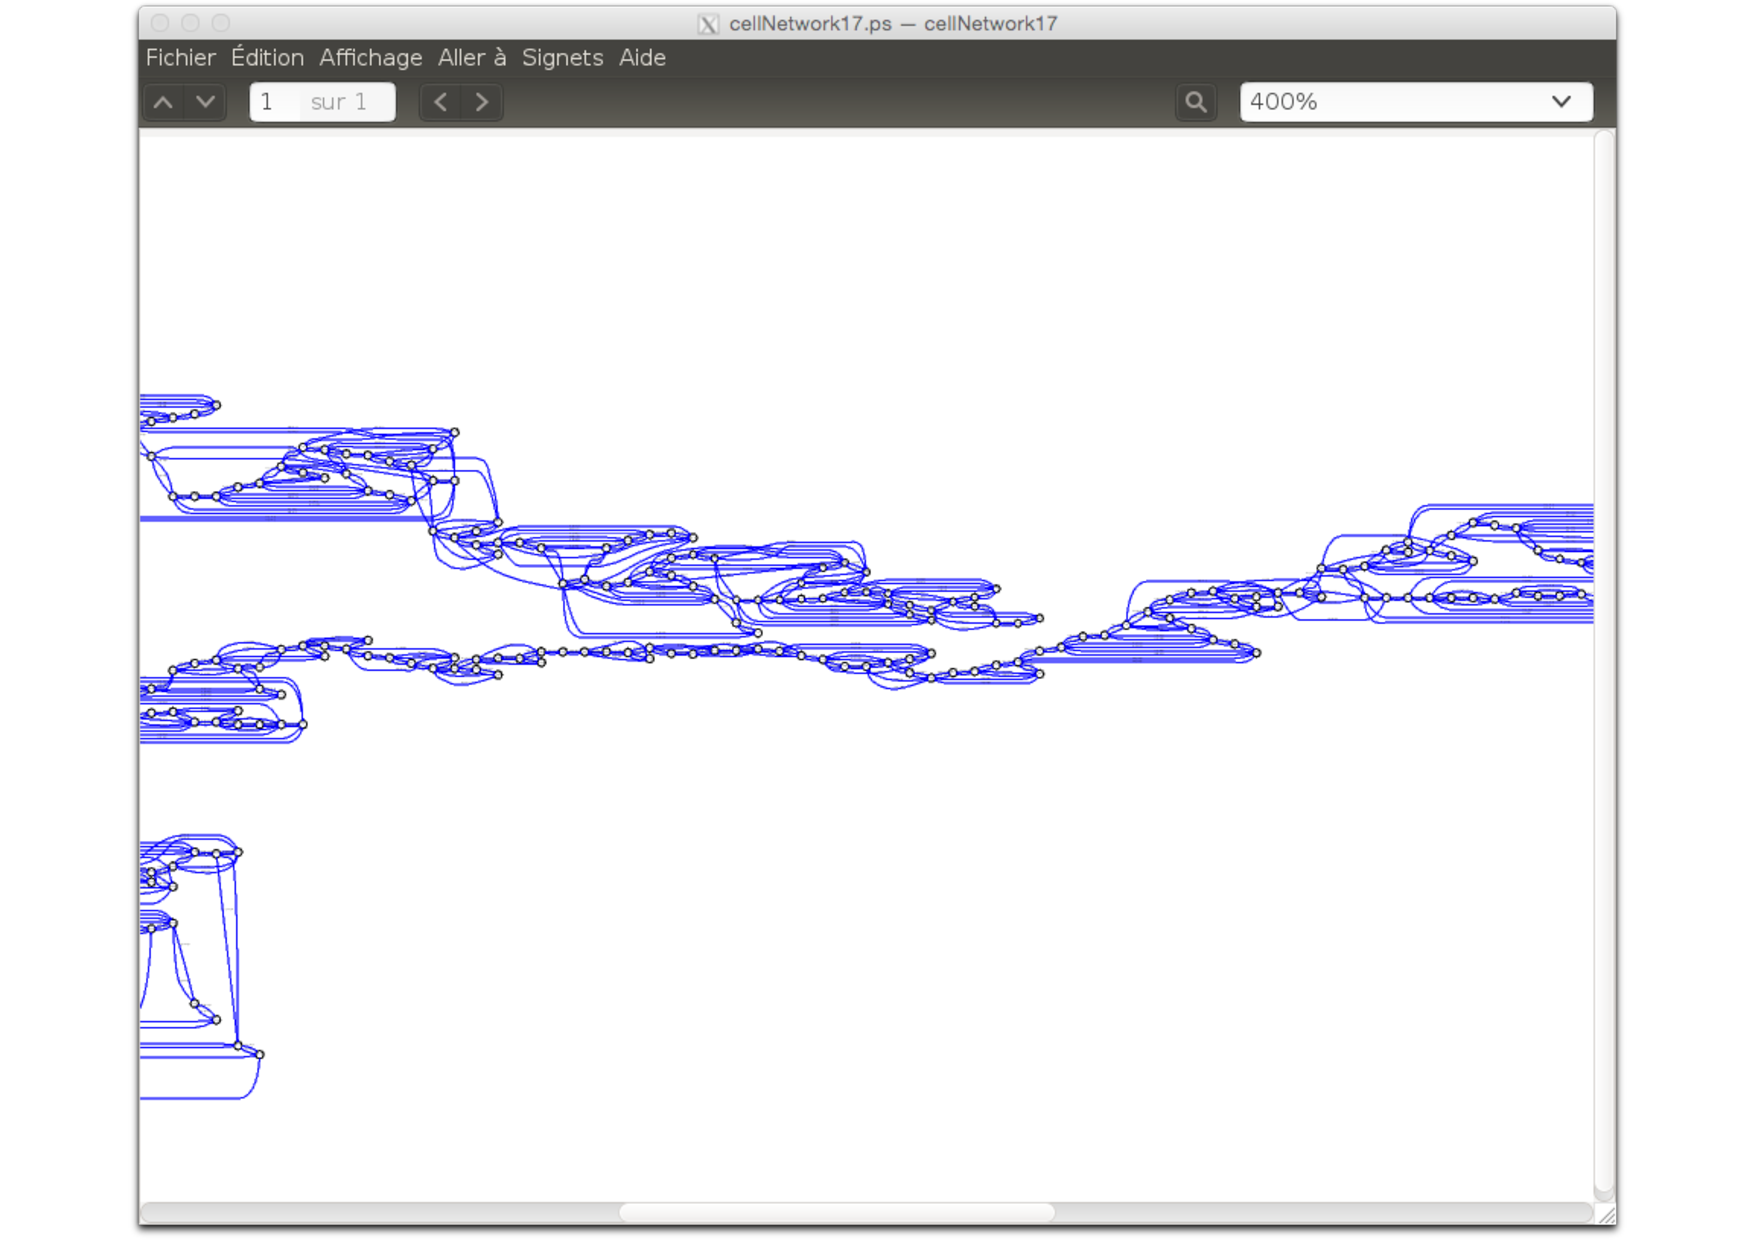
\includegraphics[width=12cm]{Diego2Networks.pdf}
\caption{View on the logic graph..}
\label{fig:antisrananaClass17bis}
\end{center}
\end{figure}


\tableofcontents
\end{document}

